%%%%%%%%%%%%%%%%%%%% author.tex %%%%%%%%%%%%%%%%%%%%%%%%%%%%%%%%%%%
%
% sample root file for your "contribution" to a contributed volume
%
% Use this file as a template for your own input.
%
%%%%%%%%%%%%%%%% Springer %%%%%%%%%%%%%%%%%%%%%%%%%%%%%%%%%%

% RECOMMENDED %%%%%%%%%%%%%%%%%%%%%%%%%%%%%%%%%%%%%%%%%%%%%%%%%%%
\documentclass[graybox]{svmult}
% choose options for [] as required from the list
% in the Reference Guide
\usepackage{mathptmx}       % selects Times Roman as basic font
\usepackage{helvet}         % selects Helvetica as sans-serif font
\usepackage{courier}        % selects Courier as typewriter font
\usepackage{type1cm}        % activate if the above 3 fonts are
                            % not available on your system
%
\usepackage{makeidx}         % allows index generation
\usepackage{graphicx}        % standard LaTeX graphics tool
                             % when including figure files
\usepackage{multicol}        % used for the two-column index
\usepackage[bottom]{footmisc}% places footnotes at page bottom
%\PassOptionsToPackage{hyphens}{url}
%\usepackage{fullpage}
\usepackage{url}
\usepackage{hyperref}
\usepackage{doi}
%\usepackage{natbib}
\usepackage{amssymb}
\usepackage{epstopdf}
\usepackage{wrapfig}
%\DeclareGraphicsRule{.tif}{png}{.png}{`convert #1 `dirname #1`/`basename #1 .tif`.png}
% see the list of further useful packages
% in the Reference Guide

\makeindex             % used for the subject index
                       % please use the style svind.ist with
                       % your makeindex program
\newcommand{\putabstract}{ Musical performances with touch-screen
  devices can be recorded by capturing a log of touch interactions.
  This object can serve as an archive or as a basis for other
  representations of the musical work. This chapter presents a protocol
  for recording ensemble touch-screen performances and details the
  processes for generating visualisations, gestural classifications,
  and graphical scores from these logs. Our experience of using these
  new representations to study a series of improvised ensemble
  performances with iPad-based digital musical instruments leads us to
  conclude that these new-media artefacts allow
  unique insights into ensemble interactions, comprehensive archiving
  of improvised performances, and the potential for resynthesis into
  new performances and artworks.}
%%%%%%%%%%%%%%%%%%%%%%%%%%%%%%%%%%%%%%%%%%%%%%%%%%%%%%%%%%%%%%%%%%%%%%%%%%%%%%%%%%%%%%%%%

\begin{document}

\title*{A Percussion-Focussed Approach to Preserving Touch-Screen Improvisation}

% Use \titlerunning{Short Title} for an abbreviated version of
% your contribution title if the original one is too long
\author{Charles Martin and Henry Gardner}
% Use \authorrunning{Short Title} for an abbreviated version of
% your contribution title if the original one is too long
\institute{Charles Martin \at Research School of Computer Science, The
  Australian National University, Canberra,
  \email{charles.martin@anu.edu.au} \and 
  Henry Gardner \at
  Research School of Computer Science, The Australian National
  University, Canberra, \email{henry.gardner@anu.edu.au}}

\maketitle
\abstract*{\putabstract}
\abstract{\putabstract}

\section{Introduction}

As an artistic experience, musical performance is fleetingly temporal
and the history of music abounds with technologies and traditions to
grab hold of musical performances, recording them in some format to be
archived, understood, and developed. All of our traditions of musical
recording, from notation, to the phonograph, to digital audio, have
contributed to the ability of performers to create new musical works
and to the place of music in our cultural landscape.

While western classial music is often defined by the
score~\cite{Davies:1991tw}, and popular music by the song or the
recorded version~\cite{Kania:2006kx}, the practice of free
improvisation often defies the identification of a canonical ``musical
work''. In free-improvised ensemble music, all decisions about the
notes to play are made in the moment by individual musicians with the
work ending only when all performers have stopped
playing~\cite{Cahn:2005uq}. With each performance equally identifiable
as a different work, the output of free-improvisation ensembles is
often represented as audio recordings with liner notes that document
changes in personnel or instrumentation. These notes are frequently
the main indicator of difference between works. Such archives of
free-improvised performances can be time-consuming to browse due to
the temporal nature of the recordings and difficult to analyse,
particularly when performers use similar-sounding electro-acoustic
instruments. When performing with computer-based instruments, however,
musicians have the opportunity to record a musical work in an
extremely detailed form by capturing a log of their interactions as
well as audio or video recordings. The log itself can serve as a kind
of score but also affords the creation of other representations of the
performance giving curators of free-improvisation new perspectives on
the musical works and the improvisers, themselves, ways to develop and
preserve their artistic practice.

In this chapter, we present a protocol for automatically documenting
performances of free-improvised music made on touch-screen computers.
Our protocol, and the touch-screen instruments with which it is used,
are designed from a percussionist-centred perspective. Rather than
particular notes and rhythms, the focus of traditional musical
notation, our protocol records detailed touch movements in absolute
time and abstract touch gestures identified during the performance by
our computer software. Given that ensemble interactions are one of the
most interesting aspects of free-improvised music~\cite{Borgo:2006fv},
our protocol is designed to connect to multiple touch-screen devices
engaged in ensemble performance over a local network or the internet.

We argue that our protocol can serve as an archival format and
addresses many of the issues with curating improvised music. We also
argue that these recorded logs satisfy Manovic's principles of new
media objects~\cite{Manovich:2002ly}; their numerical representation
allows them to be automatically varied and transcoded into new
artifacts allowing new characterisations, analysis, and appraisal of
performances. Statistical analysis of the logs can abstract the form
of improvisations away from particular instruments and players,
providing a broader understanding than can be gained from audio
recordings. Algorithmically generated visualisations and gestural
scores created from the logs leads to new perspectives on our
performances and feeds back in to the process of developing an
improvised practice.

We will describe our protocol for capturing touch interactions and how
it has developed from previous schemes for capturing and controlling
musical performances. We will also present the classification and
visualisation tools used for analysing and comparing performances
documented with our protocol. Our protocol and these tools were
developed as part of a series of research projects in touch-screen
musical performance and we will discuss how they have influenced the
research and artistic outcomes of these projects. In particular, we
will discuss the experiences of using these systems with Ensemble
Metatone, a free-improvisation percussion group that participated in a
longitudinal study over eighteen months performing with our
touch-screen instruments.

% ~\cite{Manovich:2002ly}
% Numerical Representation
% Modularity - 
% Automation - 
% Variability - alternative representations
% Transcoding - interactive cultural and computer layers, the computer
% layer can influence the cultural.


\section{Percussive Improvisation on touch-screens}
\label{sec:percussive-interaction}

The development of our touch-screen instruments and performance
logging protocol was a percussionist-centred process. Performances and
rehearsals of Ensemble Metatone, a free-improvising percussion
ensemble, were conducted to explore and evaluate instruments. Our
performance logging protocol was developed over this process to
document and analyse these activities. The same instruments and tools
were introduced to other experienced percussionists for subsequent
performances and have only been used with non-percussionists
relatively recently. Before detailing the protocol and instruments, it
is worth considering why percussive improvisation is a useful process
for characterising musical interaction.

Percussion is an artistic practice defined by an approach to
interaction rather than by any particular instrument that
percussionists play. Percussionists perform by ``striking, scraping,
brushing, rubbing, whacking, or crashing any... available
object''~\cite{Schick:2006fk}. Blades~\cite{Blades:1992kx} discusses
the earliest percussion instruments, idiophones, where the body of an
instrument creates the sound, rather than an air column or string. He
divides them by their method of interaction: ``shaken'', ``stamping''
(played with the hands or feet), ``scraped'', ``concussion'' (two
parts struck together), and ``struck'' (with a stick or non-sounding
implement). These descriptions match taxonomies of modern instruments
(such as Cook~\cite{Cook:1997vn}) and focus on the mode of interaction
for the instruments rather than their physical design.

Modern percussionists are accustomed to exploring non-traditional
objects to create music and use these percussive gestures to coax wide
varieties of timbres and musical gestures from simple instruments.
Performers of Xenakis' \emph{Psappha}~\cite{Xenakis:1975uq} or
Feldman's \emph{King of Denmark}~\cite{Feldman:1965uq} must design
their own multi-instrument setup to fit the composer's specifications.
To meet the requirement for metal instruments, for example, a
performer might find a car's suspension spring, a saw-blade or create
a unique object from scratch. This percussive approach to
investigating new instruments can be applied to touch-screen computers
which can also be struck, scraped, and rubbed with fingers and hands.

\subsection{Composing with Gestures}
\label{subsec:composing-gestures}

\begin{figure}
\begin{center}
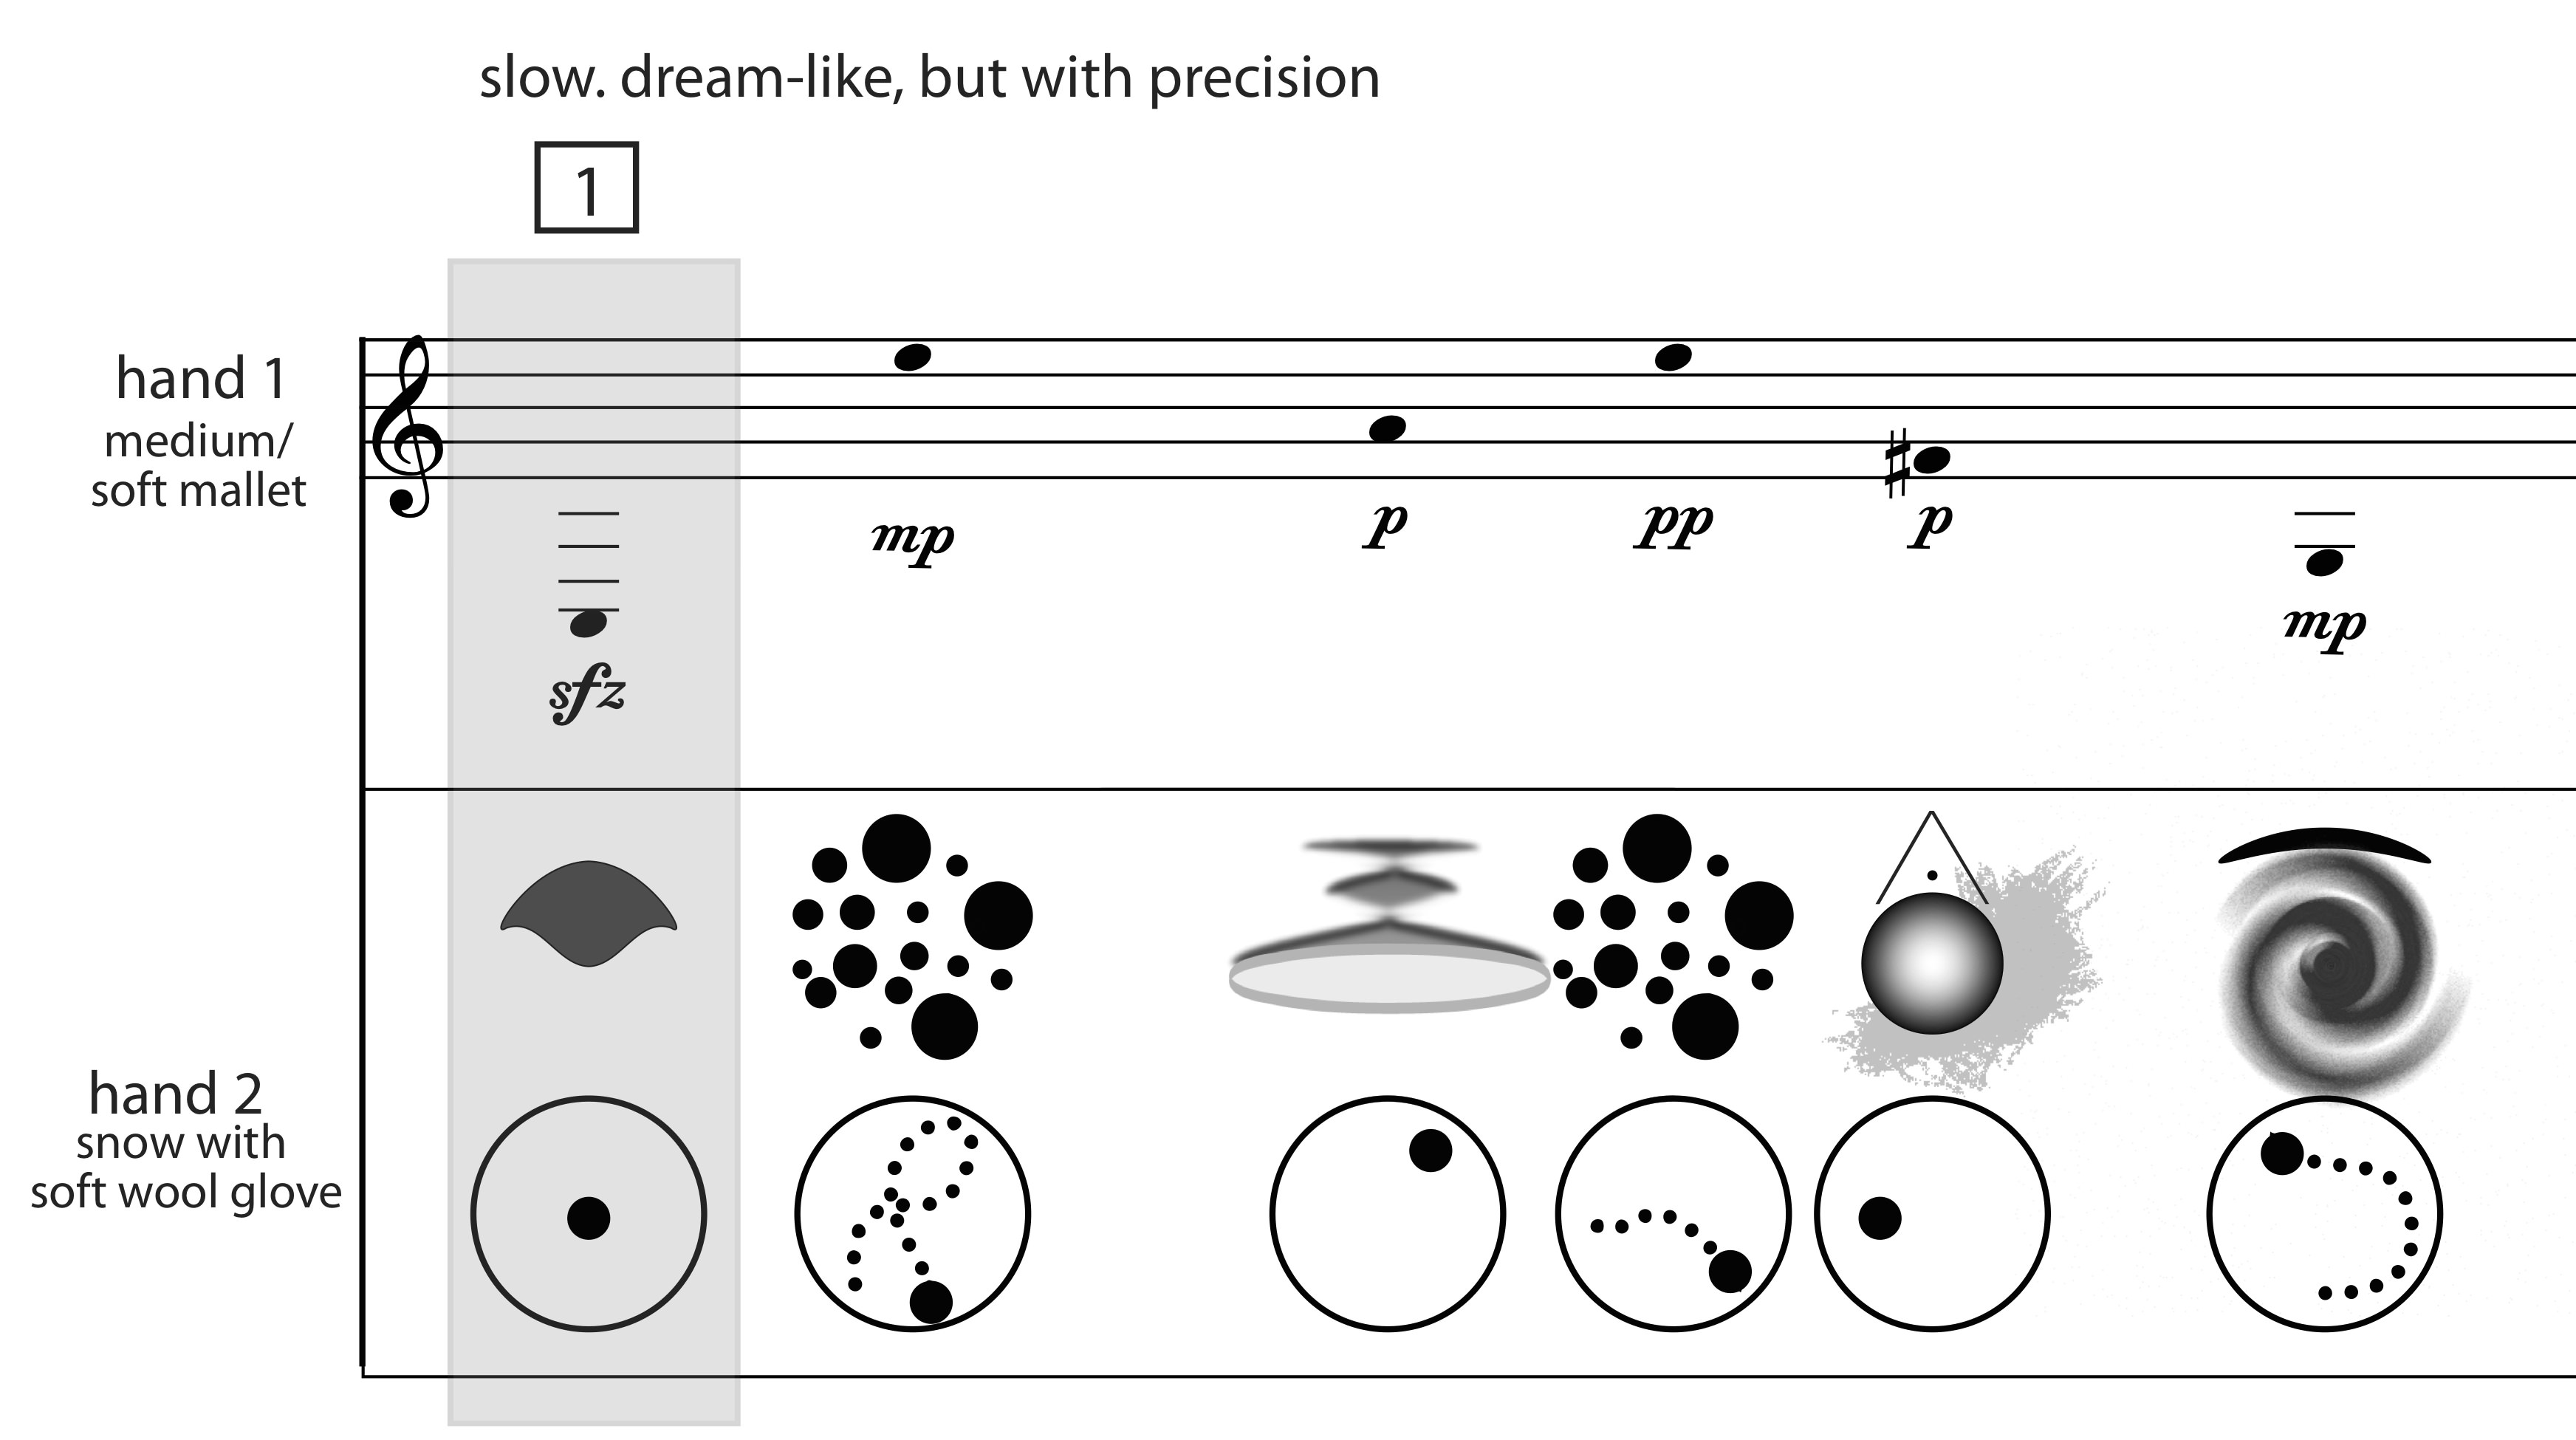
\includegraphics[width=0.7\columnwidth]{figures/syntaxofsnow-excerpt-bw}
\end{center}
\caption{An excerpt from Matthew Burtner's \emph{Syntax of
    Snow}~\cite{Burtner:2011fk} for solo glockenspiel and bowl of
  amplified snow. The composer defines a vocabulary of
  gestures for interacting with the snow with one hand represented by
  symbols below a regular staff for notes on the glockenspiel.}
\label{fig:SyntaxOfSnow}
\end{figure}

While traditional musical notation specifies sonic outcomes - pitch,
articulation and rhythm - it is possible to compose music by
specifying gestures used for interacting with instruments. For
percussionists, where gestures are transported across a variety of
instruments, this is a popular way of notating music for particularly
unconventional instruments. Thierry de May's \emph{Music
de Tables}~\cite{May:1987fk} is written for three percussionists who
perform on the surfaces of regular tables. de May defines a vocabulary
of notation for gestures that are used with standard rhythmic notation
in the score. Burtner's \emph{Syntax of Snow}~\cite{Burtner:2011fk}
asks the solo performer to play a glockenspiel with one hand and a
bowl of snow with the other. The score sets out a complex scheme of
gestures for ``playing'' the snow, with a pair of symbols (see Figure
\ref{fig:SyntaxOfSnow}) for each gesture, representing the type of
gesture as well as hand position in the bowl. 

% \begin{table}\centering
% 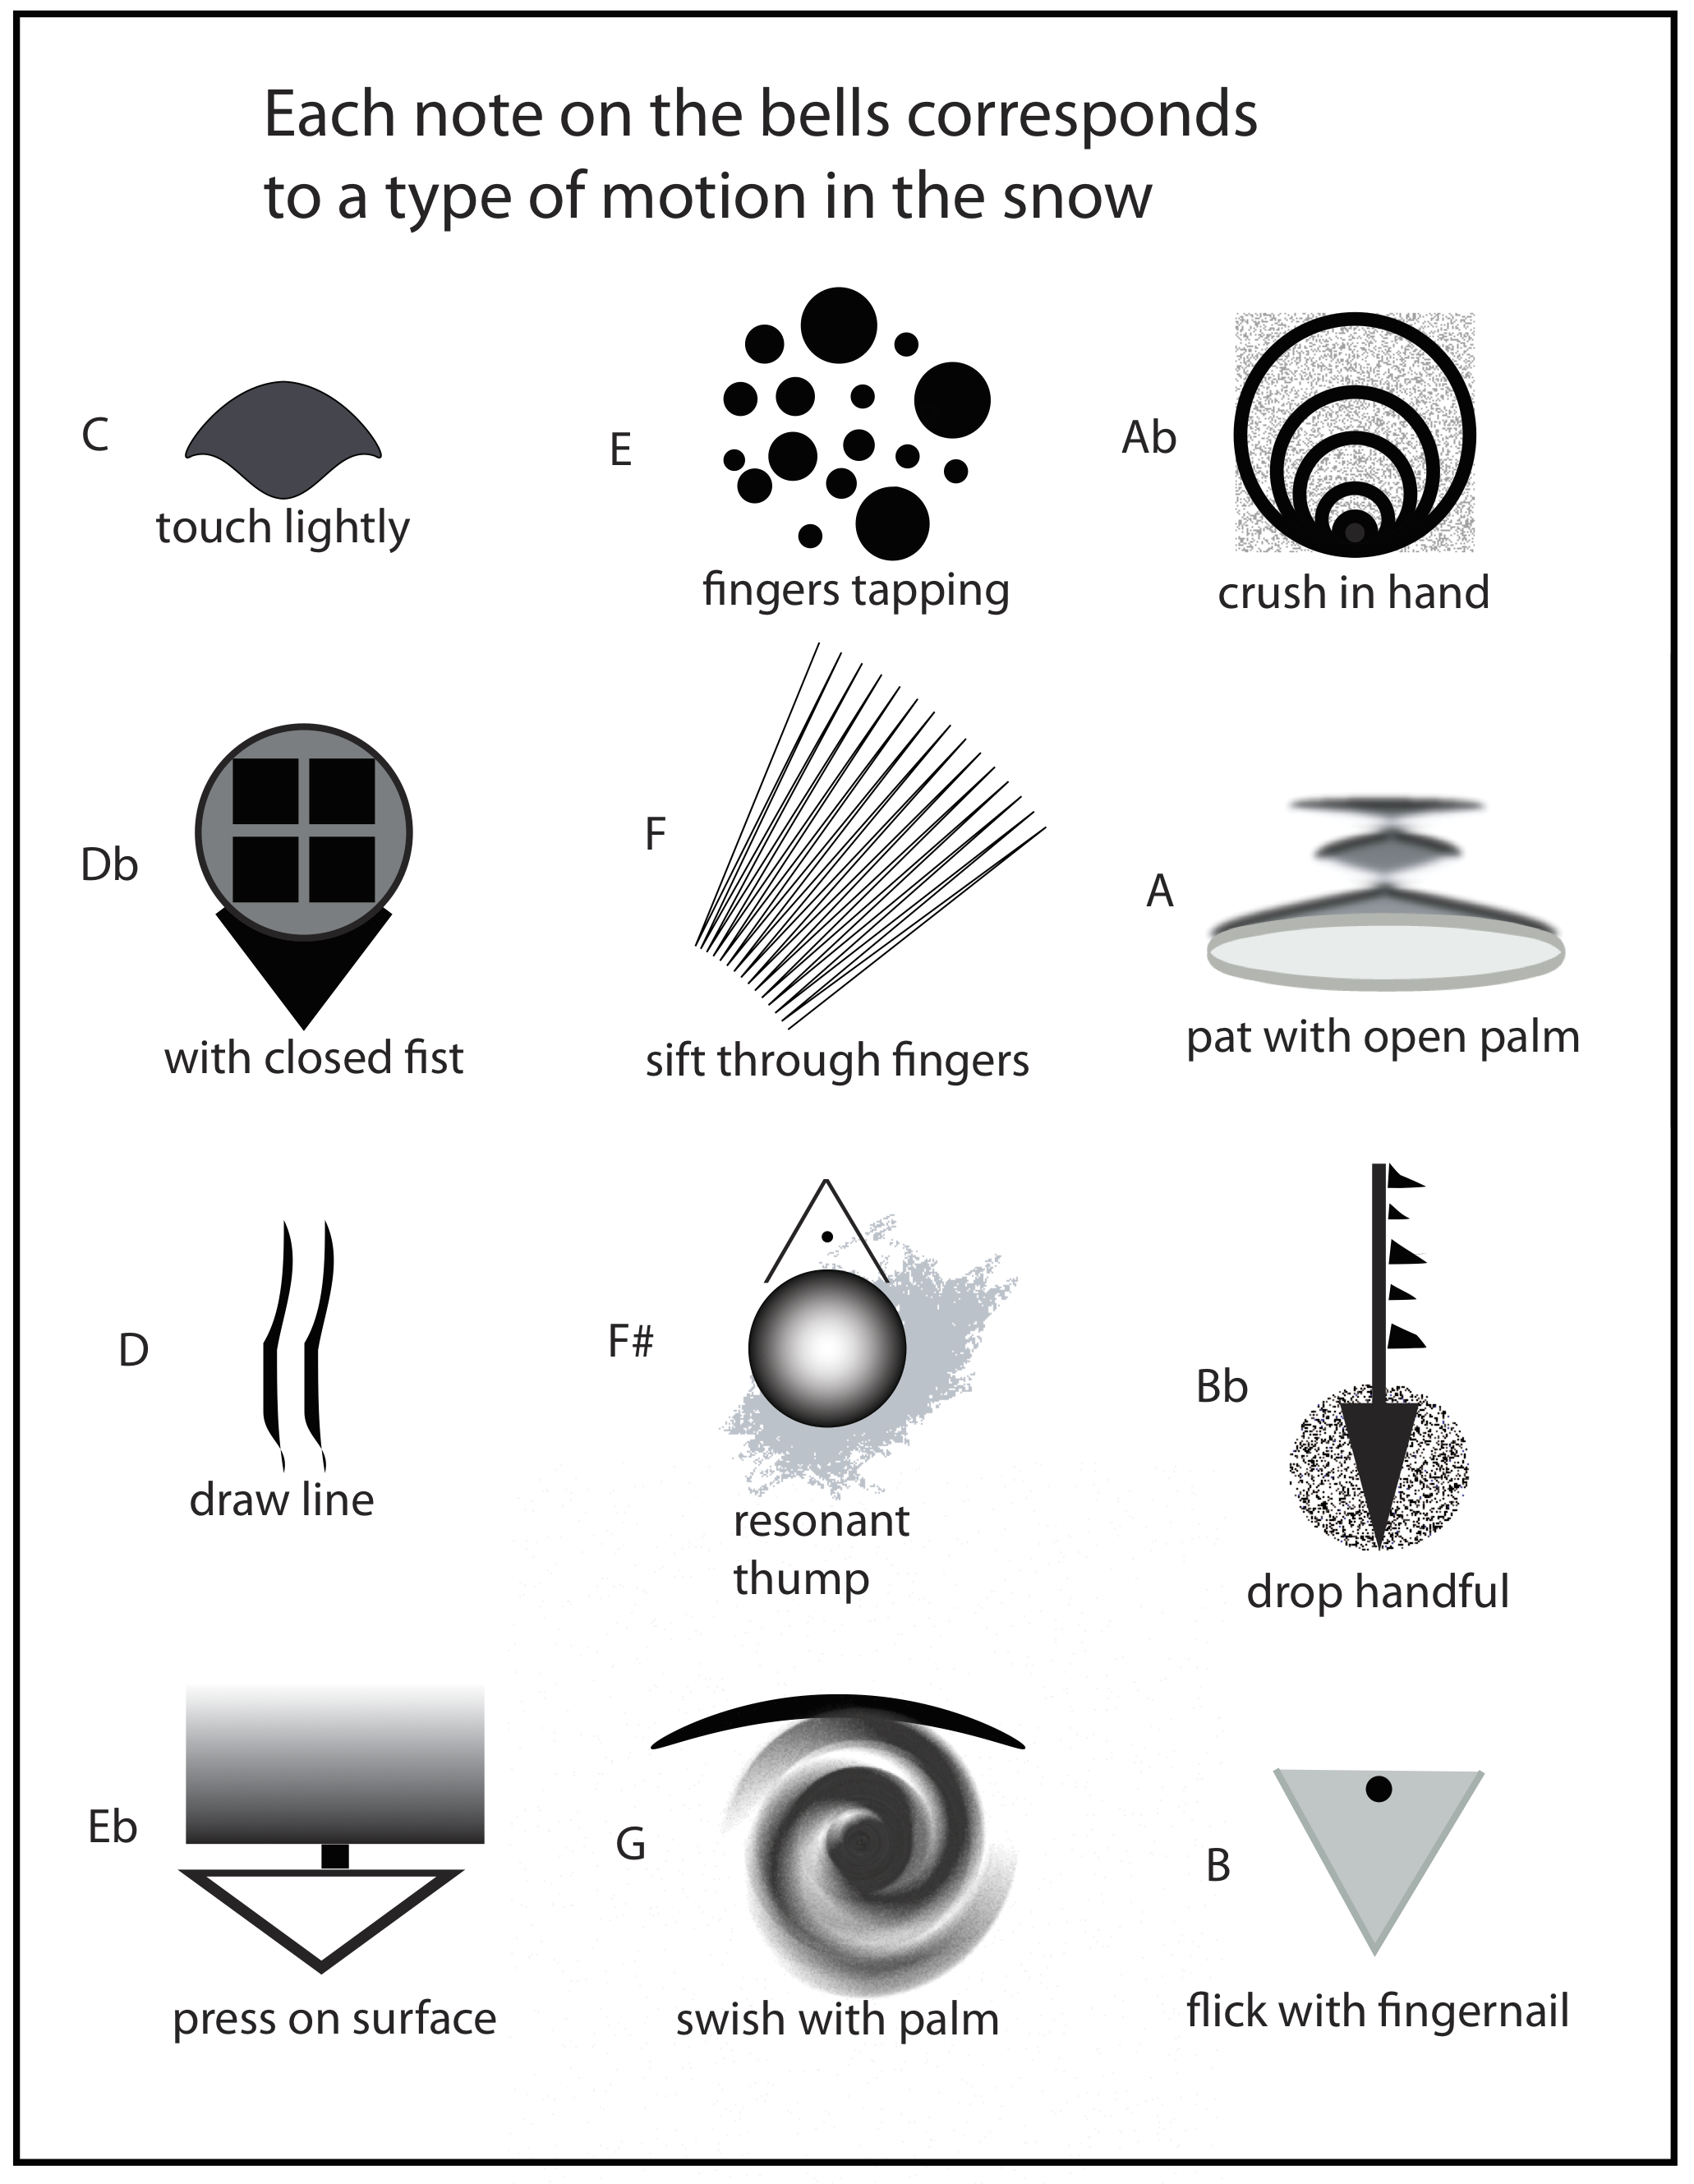
\includegraphics[width=0.4\columnwidth]{figures/syntaxofsnow-vocabulary}
% % \begin{tabular}{|l|}
% % \hline
% % touch lightly \\
% % fingers tapping \\
% % sift through fingers \\
% % with closed fist\\
% % crush in hand\\
% % pat with open palm\\
% % drop handful\\
% % flick with fingernail\\
% % draw line\\
% % resonant thump\\
% % press on surface\\
% % swish with palm\\
% % \hline
% % \end{tabular}
% \label{tab:SyntaxOfSnowGestures}
% \caption{The vocabulary of gestures to perform on the amplified snow
%   in Burtner's \emph{Syntax of Snow}. Each gesture is represented by a
%   symbol in the score and are played simultaneously with notes on the glockenspiel.}
% \end{table}

Although Burtner's vocabulary of gestures is specific to the
particular case of performing with snow, some of the gestures (e.g
``touch with finger'', ``swish with palm'', ``draw line'') could
generalise to other instruments and to touch-screens. For documenting
performances on touch-screens it is necessary to characterise a
vocabulary of gestures that is common to many different types of
instruments that can be implemented on touch-screen devices and can
express a wide variety of playing styles.

It is notable that many of the gestures indicated in Burtner's score
could be interpreted as being continuous rather than ceasing after a
following the instruction. For example, ``fingers tapping'' should
probably be interpreted not as one or two taps but as a continual
tapping until the performer reaches the next instruction. In HCI
research, gestures on touch-screens are frequently characterised as a
having a short and finite expression such as the ``unistroke''
gestures described by Wobbrock et al.~\cite{Wobbrock:2007kq}. These
gestures are usually designed to execute a command in software (e.g.
double tap to open a menu) rather than to create an artistic
expression. For this reason, characterisations of touch gestures that
already exist in the HCI literature are unsuitable for characterising
performative touch gestures which mainly consist of continuous
interactions.

% While these devices can be configured with a wide variety of software
% with many different kinds of sonic output (we discuss several of our
% own apps in Section \ref{subsec:metatone-apps}), the touch-screen and
% its gestural affordances always remains the same. As a result, even
% though a sonic characterisation may be limited to individual apps, the
% percussive gestures can be general enough to understand performances on
% different apps and even different devices.

% The gestures, which
% include ``fingers tapping'', ``swish with
% palm'', ``draw line'', and ``sift through fingers'', are often open
% with respect to the exact location, shape, and length of the
% interaction. 


\subsection{Free-Improvised Performance}
\label{subsec:free-improvisation}

Free improvised performance has been defined as the performance of
music ``without any restrictions regarding style or genre and without
having predetermined what is to be played''~\cite{Stenstrom:2009xy}.
This definition is a typical of the field, but it frames
free-improvisation subtractively: improvisation is ``regular''
performance minus restrictions. To understand what is really exciting
about free-improvisation as a mode of artistic expression and as a
methodology for researching unfamiliar interactions, we must look at
what free-improvisation \emph{adds} to performance. Bill Cahn, member
of the pioneering percussion group, Nexus, writes that improvisation
encourages ``a deeper knowledge of the instruments and their
sound-making possibilities''~\cite{Cahn:2005uq}. Digital media
theorist Aden Evens writes that when improvising with an unfamiliar
instrument ``the musician generates novel and surprising results even
when applying familiar technique.''~\cite{Evens:2005kx}

Although it is rare for free-improvisations to be subjected to an
internal musical analysis, unlike other forms of music including jazz
improvisations, some characterisations of the internal structure of
these performances have been published.
Pressing~\cite{Pressing:1988uo} has developed a model of improvisation
that divides performances into a series of non-overlapping events
separated by trigger points during the performance that initiate each
event. Stenstr\"om proposes a terminology for free ensemble
improvisation, including concepts such as ``transitions'' between
musical ideas and ``attractors'' such as a steady pulse that encourage
similar playing from other performers~\cite{Stenstrom:2009xy}.
Nunn~\cite{Nunn:1998ly} similarly argues that a ``segmented form''
divided by ``transitions'' is the fundamental structure of free
improvisation.

Much free-improvised music is performed by ensembles of performers
rather than solo artists~\cite{Stenstrom:2009xy}. In fact, definitions
of free-improvisation have emphasised this aspect with Mazzola writing
that one of the free improvisor's primary roles is ``to negotiate
(while playing) with their fellow players every single item they bring
into play... as if partaking in a dynamic and sophisticated
game.''~\cite{Mazzola:2009cr} 

\subsection{Ensemble Metatone and improvising iPad ensembles}


\begin{figure}
  \centering
  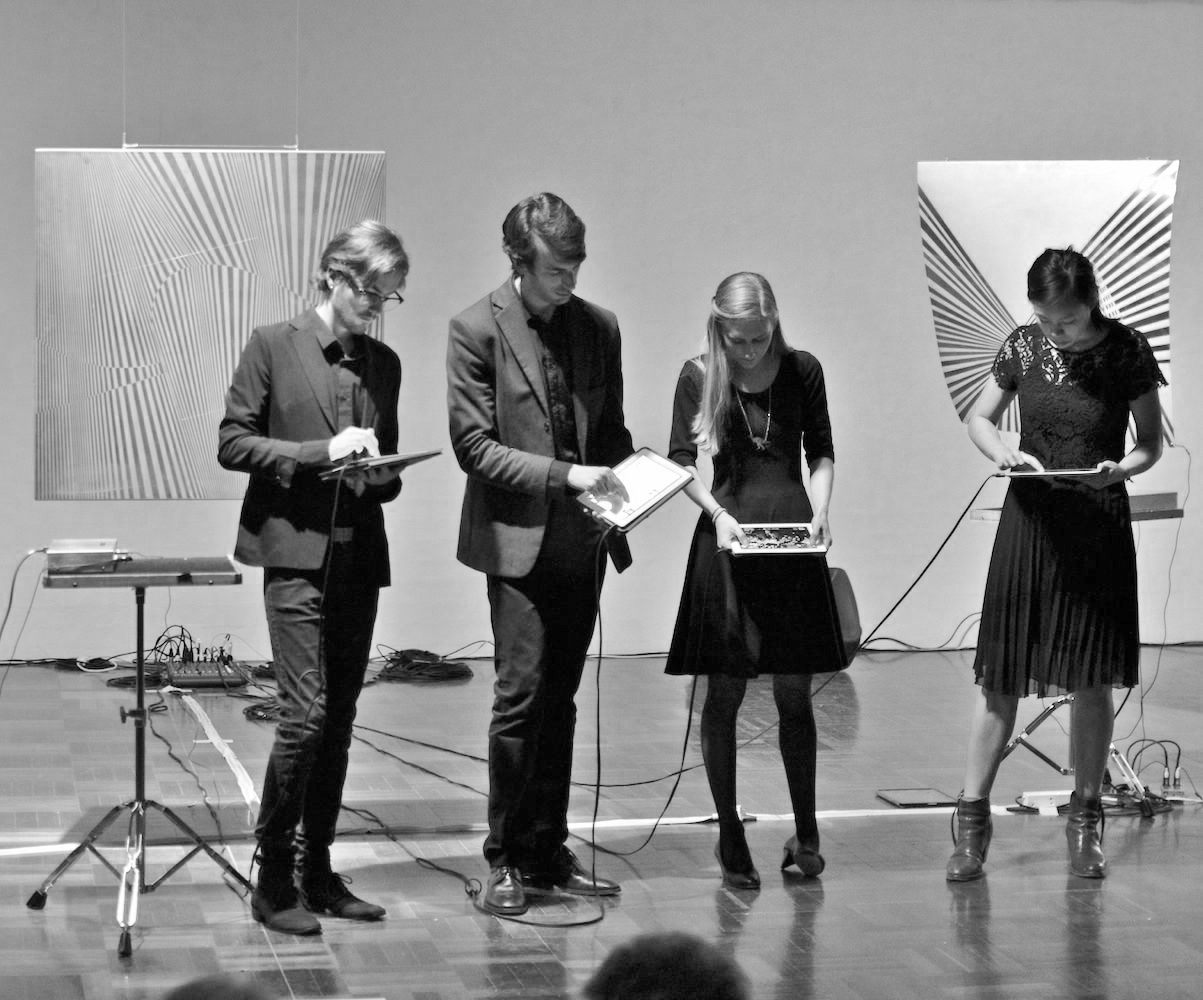
\includegraphics[width=0.5\textwidth]{figures/ensemblemetatone-bw}
  \caption{Ensemble Metatone performing \emph{MetaLonsdale} at the ANU
    School of Art Gallery in October 2013 (left to right: Jonathan
    Griffiths, Charles Martin, Christina Hopgood, Yvonne Lam).}
  \label{ensemblemetatoneperforming}
\end{figure}



In the present research, an improvising percussion group was not only
used to create new music but to explore and evaluate touch-screen
instruments running on Apple iPads. Ensemble Metatone was brought
together in Canberra, Australia to study the process of performing
free-improvised music starting with a prototype app and, through a
process of iterative design, eventually presenting concerts with
multiple apps. The members of the group (including one of the authors)
were all highly qualified in classical percussion and had significant
experience as improvisors.

Ensemble Metatone undertook a series of studio rehearsals throughout
2013 to develop a repertoire of free-improvised music with our iPad
apps~\cite{Martin:2014jk}. Using a process of ``creative music
making''~\cite{Cahn:2005uq} where improvisations are followed by
critical listening and discussion, the performers developed a
vocabulary of touch interactions inspired by their percussion
training. Notably, they also discovered novel sounds from the
instruments that could be created with unusual or atypical
interactions and were not foreseen by the app
designer~\cite{Martin:2014cr}. The performers of Ensemble Metatone
settled on a combination of iPad and acoustic percussion instruments
allowing them to choose from a wide palette of sound colours in their
performances. The initial series of rehearsals was followed by a
recorded research concert with a live audience, a series of
performances at experimental art events. The recording of Metatone's
research concert was released as a digital album in March
2014~\cite{Ensemble-Metatone:2014sf}.

Other percussion performers were also invited to work with our
touch-screen apps in a variety of improvised and semi-composed
performances in Australia and the USA. In 2014, a number of Metatone
apps were made available for free in the Apple iTunes App Store and
the authors are aware of several performances using the apps unrelated
to our work.

In 2015, the Metatone apps were used as part of the educational
activities of the New Music Ensemble at the ANU School of Music
including rehearsals and performances and in activities with
high-school students. In this setting participants had a range of
instrumental experience so iPads were used as the only instrument. A
formal study was conducted with four iPad quartets, including members
of the New Music Ensemble and volunteers from the local music
community, who performed several improvisations with different
combinations of software features.

The majority of these rehearsals and performances were audio and video
recorded and also documented using our touch-screen performance
protocol. To date, we have archived over 80 performances of our iPad
apps using these tools forming a highly comprehensive corpus of work
for studying improvisation on touch screens. In the following
sections, we will describe forms of analysis and derivative works that
can be generated from this archive of performance documentation.

\subsection{Curating the Improvised}
\label{subsec:curating}

Although the field of improvised performance has a developing
theoretical background and many highly regarded practitioners,
particular artistic expressions tend toward the ephemeral. We advocate
an expanded method of documenting improvised music that encodes not
just the sounds made in the performance space, but performers'
music-making gestures and ensemble interactions.

It is widely recognised that both musical works and new media
artefacts can have a number of interacting
representations~\cite{Rinehart:2007pi}. Musical works might be
directed by a score; might be ``thick'' or ``thin'' depending on the
the freedom of interpretation afforded the performers; be represented
in live performance, studio recordings, or by computer generated
renderings; and may be composed or improvised~\cite{Davies:2005fj}.
Combinations of these representations are often collected together to
form an archive of a musical work.

Free-improvised music, where performers do not follow a set musical
structure, is usually preserved using only audio and video recordings.
While the improvised solos of famous jazz musicians are often
transcribed, this is extremely uncommon for free-improvised ensemble
performances. Audio recordings of free-improvised performances capture
the sonic results of the performers' explorations of musical gestures
and interactions with other ensemble members but the original
performance gestures are lost. For performances with electro-acoustic
instruments, audio-recordings can be inadequate for detailed analysis
as it is often difficult to discern which musician is creating each
sound.

When improvised music is performed on touch-screen instruments, a log
of touch-interactions captured during the performance can suplement
traditional recordings and could take the place of a musical
``score''. While scores are generally used for composition, their use
as documentation for new media artworks has been
acknowledged~\cite{MacDonald:2009ve}. Such a log would also satisfy
Manovich's principles for a new media artwork~\cite{Manovich:2002ly}.
In particular, the log of touch-interactions is variable, forming the
basis for derivative artworks that also represent aspects of the
original performance.

Borgo has drawn parallels between the swarm-like collaboration in
free-improvised performances and the community collaborations that
define the field: 
\begin{quote}
``One of the particular challenges of contemporary
improvisation, for both players and listeners, is to remain aware of
and sensitive to the many musical gestures and processes circulating
between members of the group in the moment of performance and between
members of the community as ideas circulate via recordings, impromptu
meetings, and the overlapping personnel of various working
groups.''~\cite{Borgo:2006fv} 
\end{quote}
These communities of practitioners, listeners, and concert organisers
are the curators of the free-improvised music world. We argue that the
ability to thoroughly document touch-screen movements of improvising
ensembles enhances the ability of such a community to develop this
artistic practice through archiving, replaying, and re-synthesising
performances. In Sections \ref{sec:protocols} and \ref{sec:analysis},
we describe our approach to recording improvised touch-screen
performances and transforming such transcriptions into animations,
gestural scores, and new artworks. These multiple representations of
musical performance allow the curation and analysis of an emerging
improvised practice.

\section{Towards a protocol for touch-screen musical performance}
\label{sec:protocols}

% \subsection{Protocols for capturing performance data}
% \label{subsec:protocols}

Musical data has been abstracted from the temporality of performance
for centuries since the development of musical notation. Mechanical
instruments such as music boxes and barrel organs, developed in the
18th century~\cite{Fowler:1967kq}, first allowed music to be
``programmed'' rather than performed. More refined mechanical
instruments such as the ``reproducing piano'', which appeared at the
turn of the 20th century~\cite{Kapur:2005fk}, allowed a musician's
performance to be automatically transcribed and converted into a paper
``piano roll'' that could be re-played many times. All of these
technologies have had an impact in the study of music as well as its
performance. Musical notation enabled the field of musicology, where
the musical score has traditionally been priveleged as the canonical
representation of a musical work. The piano-roll performances of many
famous pianists were made before audio recording was widespread and
have been used to analyse their performance styles.

% citation for piano roll.

An important antecedent of our work was the
MIDI~\cite{midi1996complete} (Musical Instrument Digital Interface)
protocol, which was developed in the late 1970s to connect electronic
music \emph{controllers}, such electronic versions of keyboards, drums
and wind instruments and new musical interfaces such as ``THE
HANDS''~\cite{TheHandsArticle}, with electronic synthesisers or
digital recording systems. While this standard was intended as a
control interface for live performance or recording, it was subverted
by digital artists and researchers who recognised that the MIDI trace
of a musical performance could be used for other purposes. MIDI was
originally designed to be used with a physical serial connection,
however virtual MIDI connections are commonly used to connect multiple
pieces of software and to other computers over a
network\cite{Lazzaro:2004pb}.

While the success of MIDI is ongoing, the semantics of the protocol is
mostly restricted to a keyboard-and-note perspective on musical data.
The typical MIDI interactions are ``note on'' and ``note off''
messages, each of which contain a pitch and dynamic (volume) value.
Changing parameters while a note is playing can be achieved by
simultaneously sending one of a limited number of ``continuous
control'' messages while the ``note on'' is held. In an effort to
develop a semantics-free format for musical control that better
reflected the needs of modern computer music systems,
OSC~\cite{osc-nime2009} (Open Sound Control) was developed. This
standard defines a message format but with the specific content of the
messages up to the application developer. The flexibility of OSC has
contributed to its success not just in computer music, but in
professional applications such as show
control~\cite{schmeder2010best}, although it is not commonly used in
commercial electronic instruments.

Some have attempted to define protocols using OSC to standardise
interaction with certain types of interface. TUIO~\cite{TUIO_KBBC05}
is one such protocol designed for table-top interfaces where fiducial
markers and finger touches can be tracked. Unlike MIDI, TUIO does not
define the purpose of messages but communicates only information about
basic components that the designers expected would be common to most
table-top interfaces. The TUIO protocol sends groups of messages
together that encompass the state of the whole table-top interface.
Most importantly, one \texttt{set} message is sent for each object on
the surface that has changed position. A \texttt{set} message includes
identification and position information about the object being tracked
as well as precalculated data such as velocity, acceleration, and
rotation. This simplifies the requirements for software receiving TUIO
which may not have to keep track of objects in between bundles of
messages or worry about errors due to messages arriving out of order.

\begin{figure}
\begin{verbatim}
- (void)touchesBegan:(NSSet *)touches 
    withEvent:(UIEvent *)event;
- (void)touchesMoved:(NSSet *)touches 
    withEvent:(UIEvent *)event;
- (void)touchesEnded:(NSSet *)touches 
    withEvent:(UIEvent *)event;
- (void)touchesCancelled:(NSSet *)touches 
    withEvent:(UIEvent *)event;
\end{verbatim}
  \caption{Callback methods for accessing touch events in Apple
    iOS~\cite{AppleDeveloper:2015rm}. Our Metatone apps log each
    \texttt{touchesBegan}, \texttt{touchesMoved}, and
    \texttt{touchesEnded} event.}
\label{touch-event-code-listing}
\end{figure}

% \subsection{Touch Screen Data}
% \label{subsec:touch-screen-data}

As described in \ref{subsec:metatone-log} below, our protocol for
logging touch-screen performances needed to capture the fundamental
interactions occuring on the touch-screen, not how these interactions
are interpreted by the application currently running on the device. In
Apple iOS devices, data collected from the multitouch digitiser in
front of the screen is interpreted by the operating system which keeps
track of individual touches and divides the incoming data into
events~\cite{AppleDeveloper:2015rm}. Software developers can implement
a set of callback functions to access these events individually.
So-called \texttt{UIEvent}s track the state of touches on the screen -
they ``begin'', ``move'', ``end'', and may be ``cancelled'' if they
are mis-recognised. For the purposes of designing software for
free-form touch improvisation, only the first three states are of
interest. The touch-data objects described by these events have a
record of their current as well as previous location on the screen. A
value proportional to instantaneous velocity of moving touches can be
easily calculated by finding the length of the vector from the
previous location to the new.

\subsection{Metatone Apps}
\label{subsec:metatone-apps}

\begin{figure}
\begin{center}
  %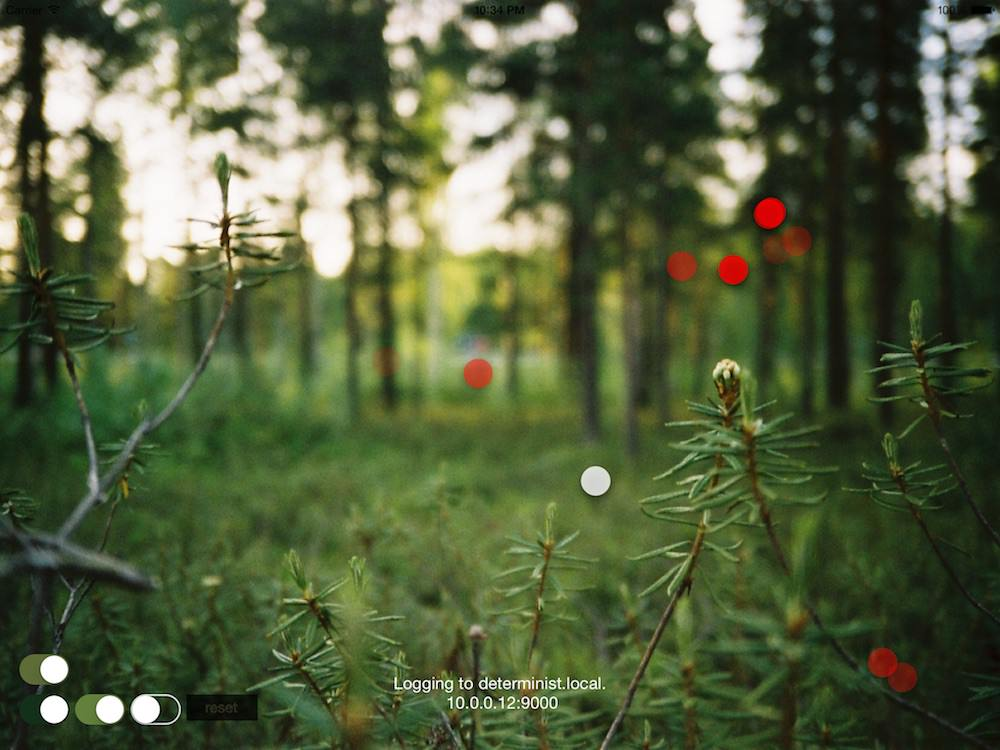
\includegraphics[width=0.45\textwidth]{figures/app-1-MetaTravels}
  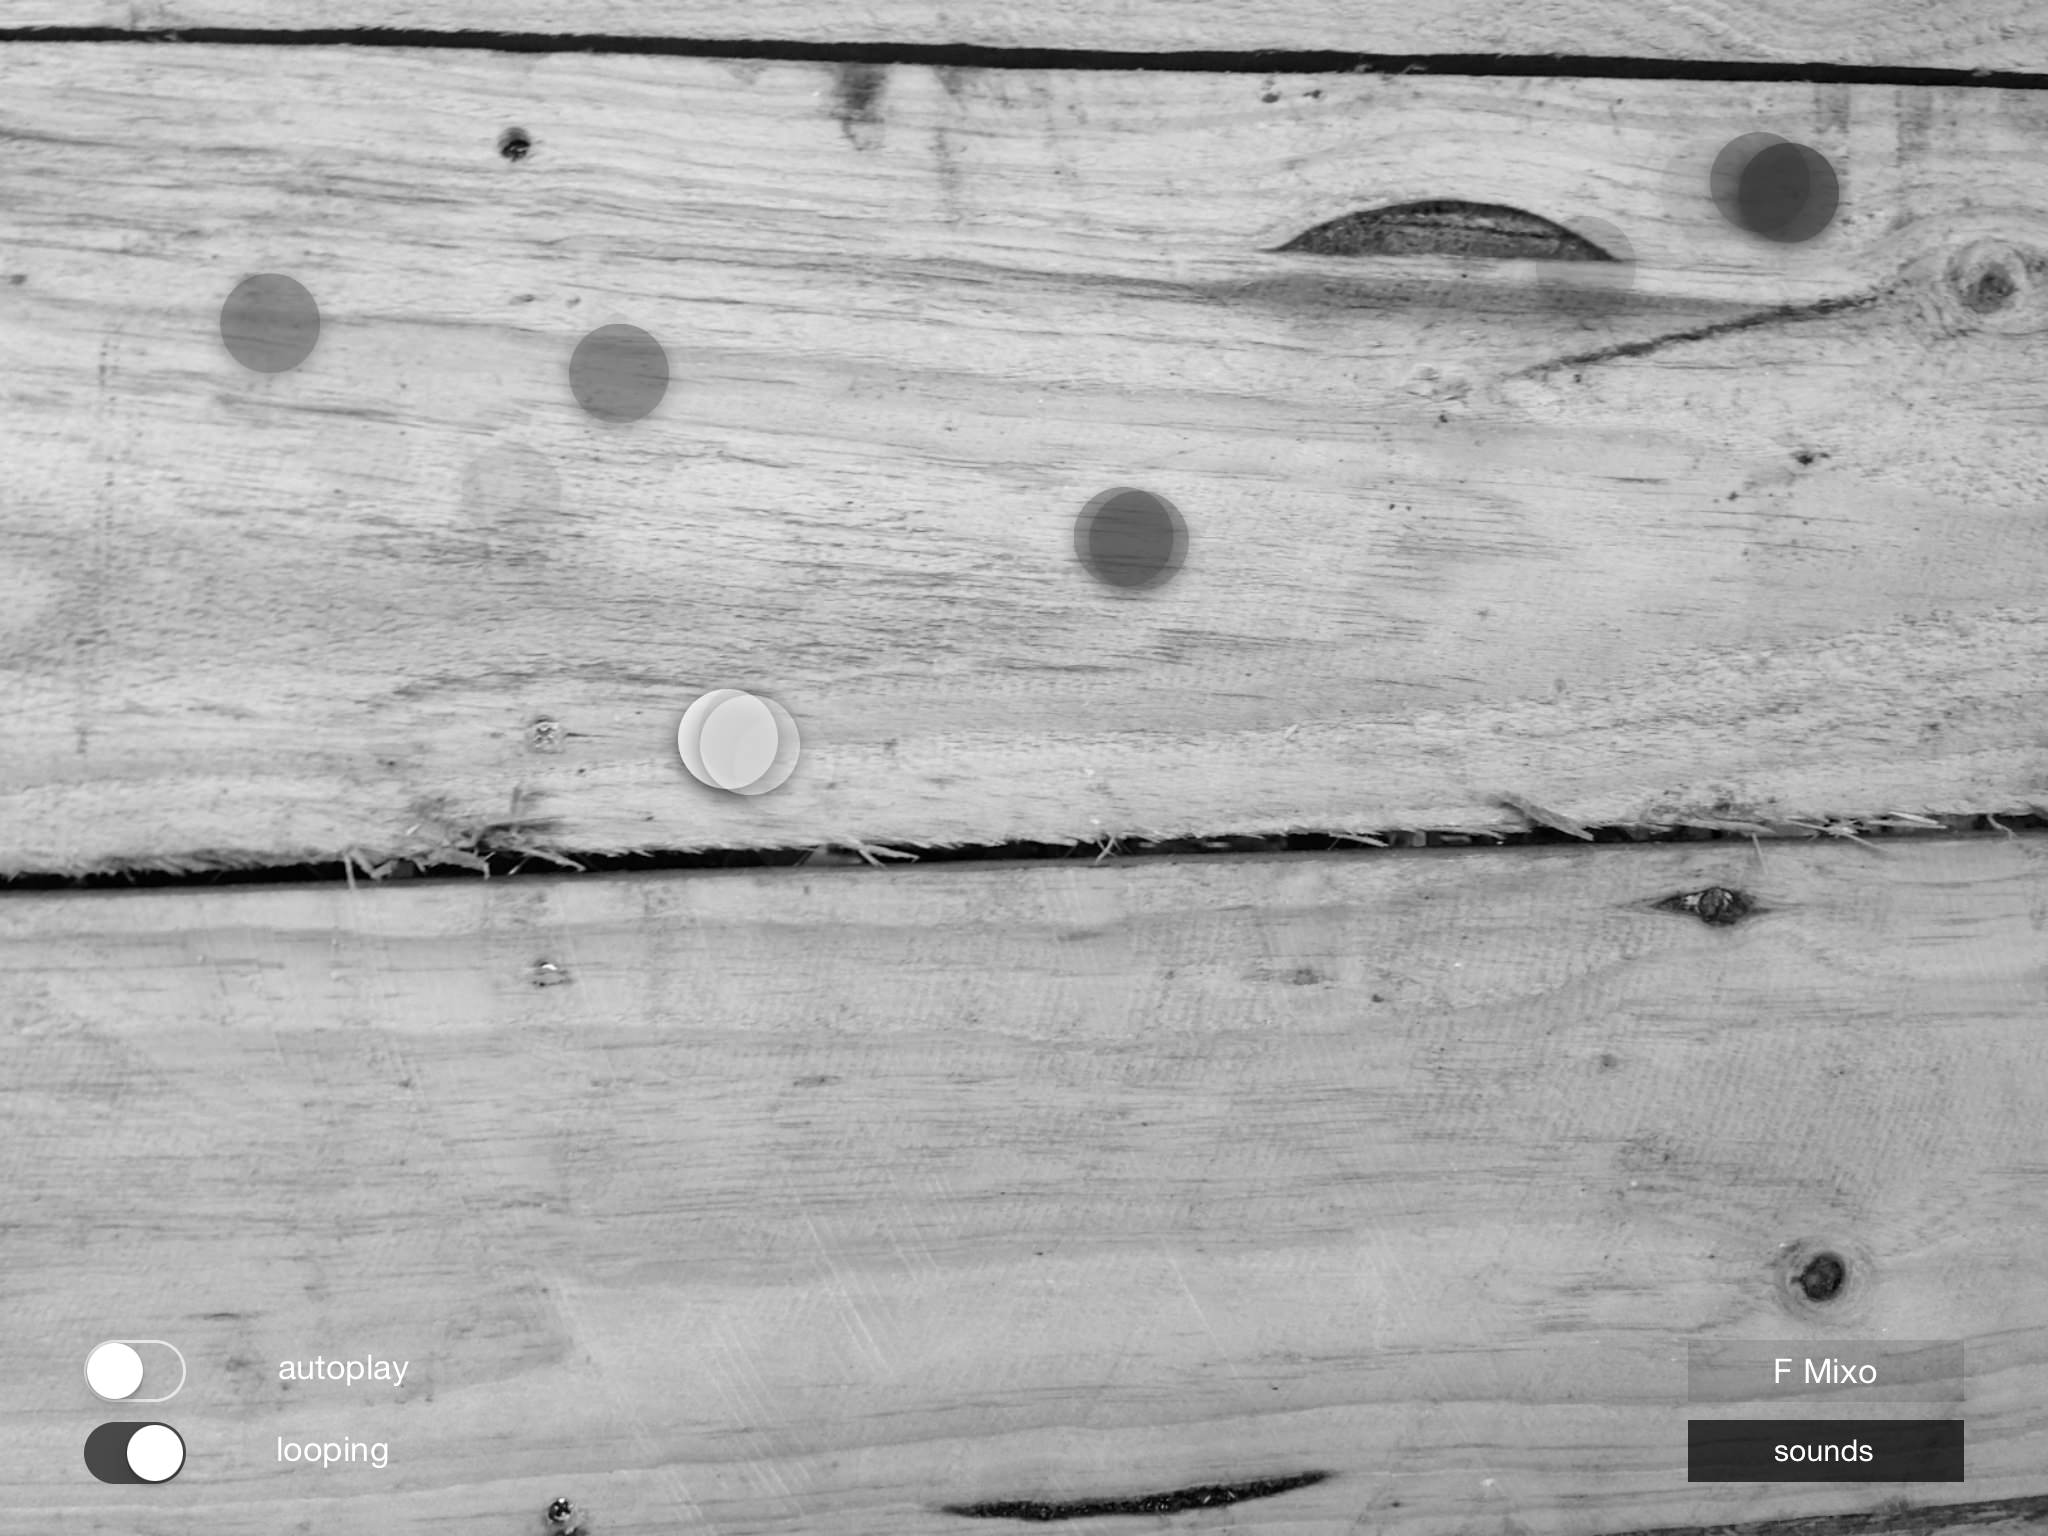
\includegraphics[width=0.45\textwidth]{figures/app-2-MetaLonsdale-bw}
  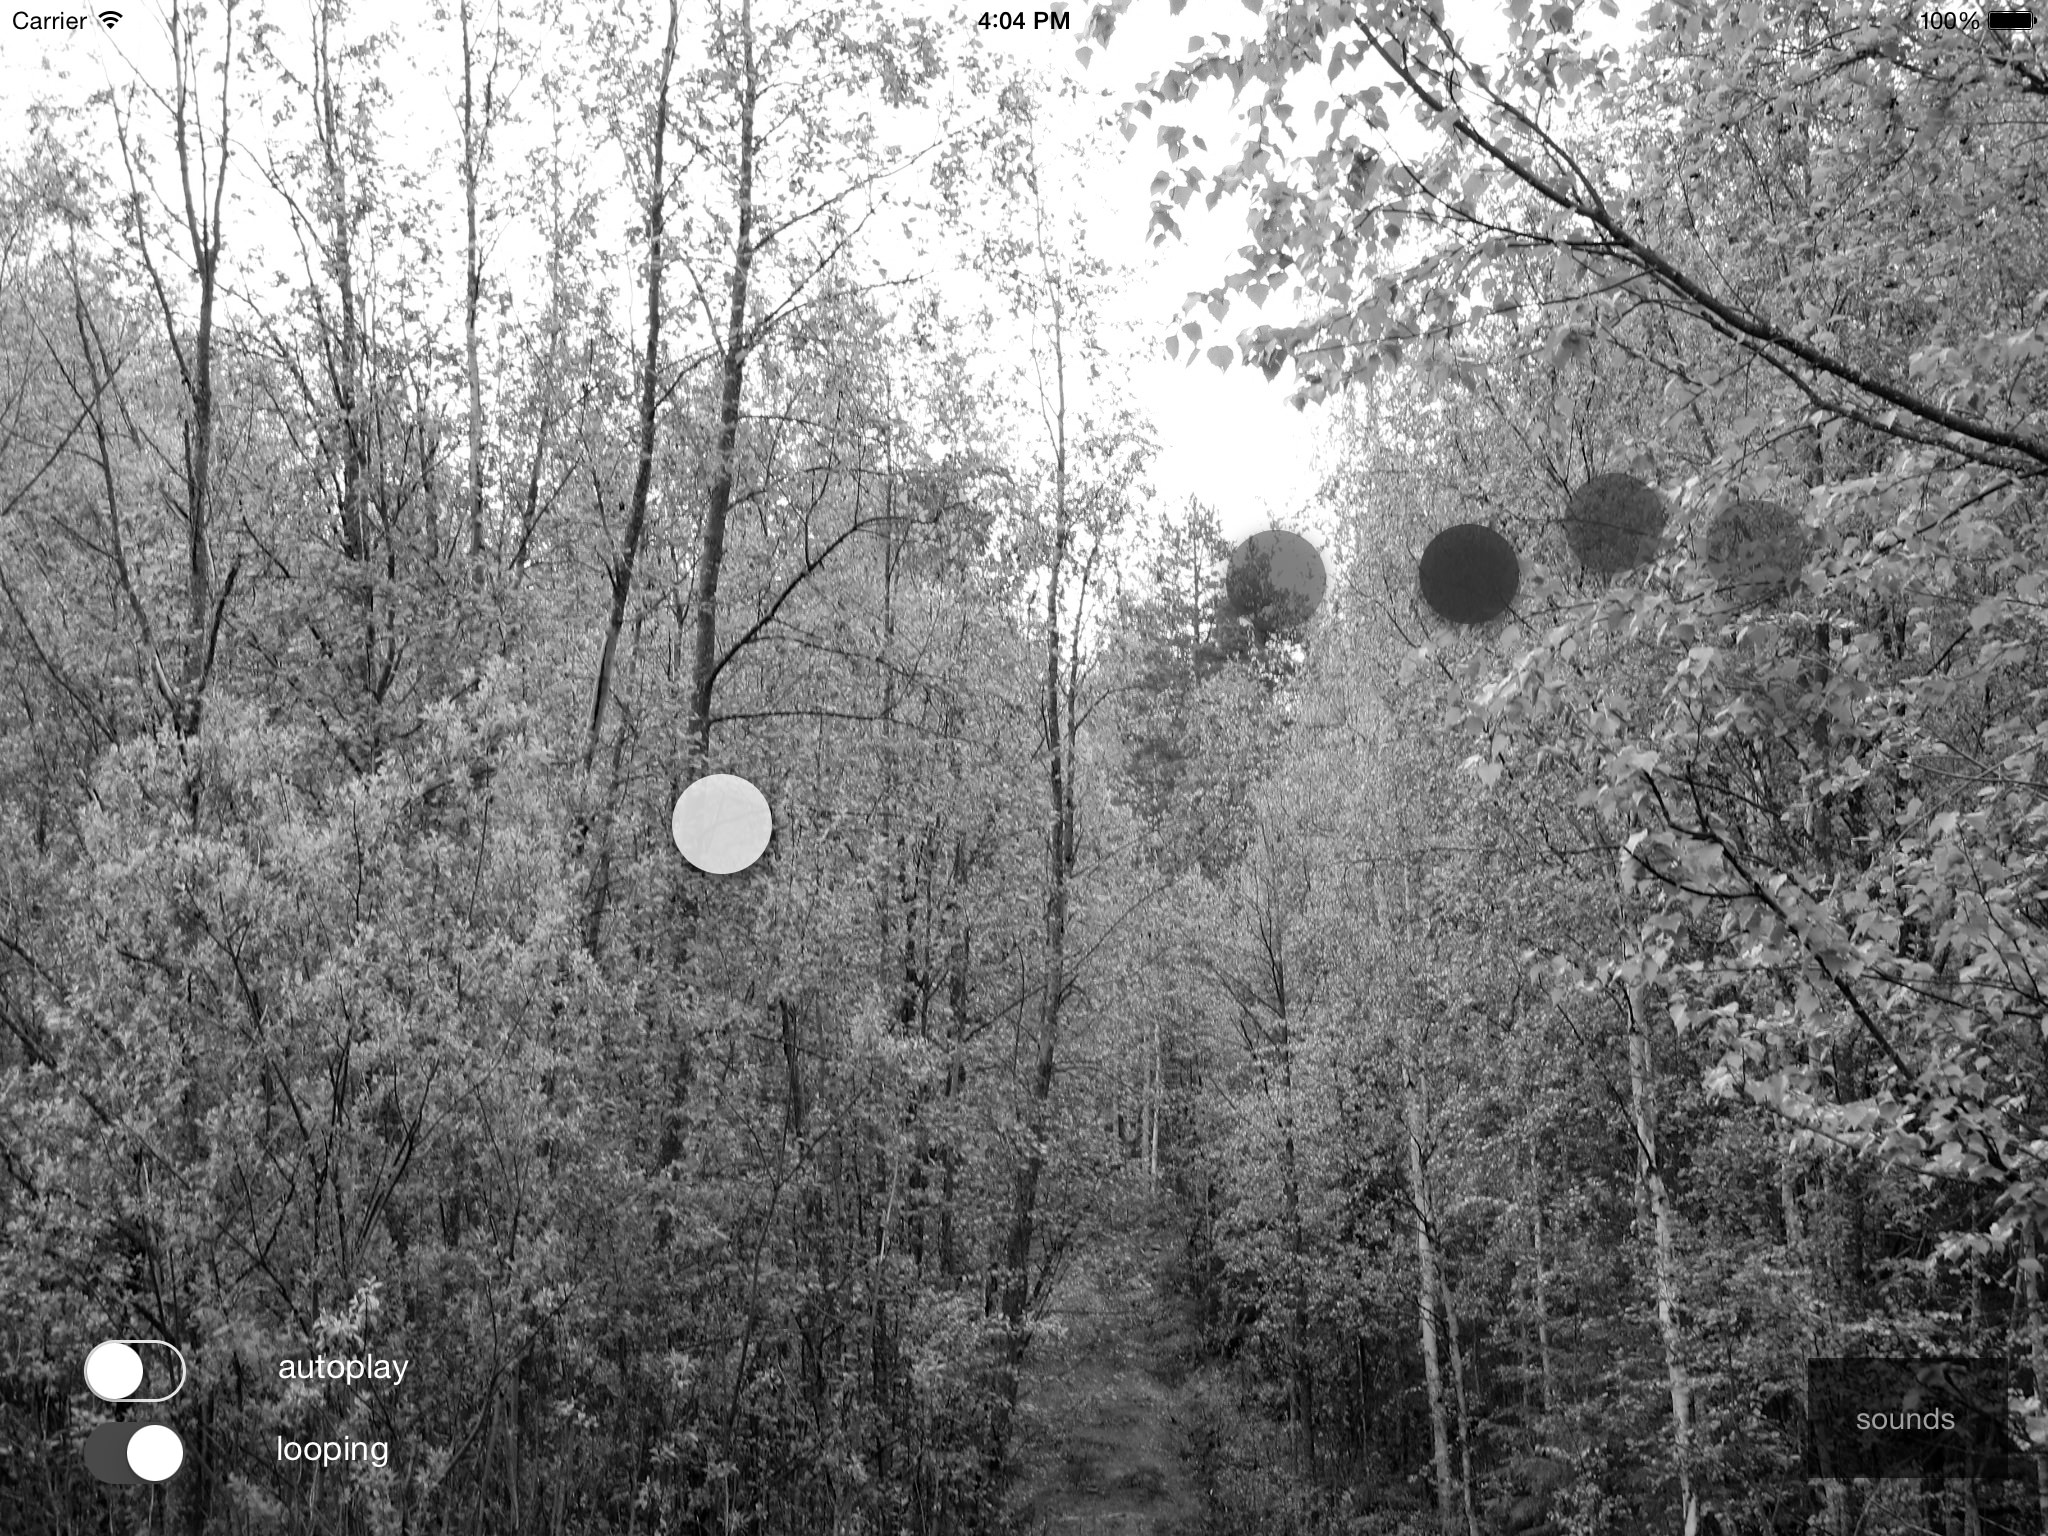
\includegraphics[width=0.45\textwidth]{figures/app-3-BirdsNest-bw}
  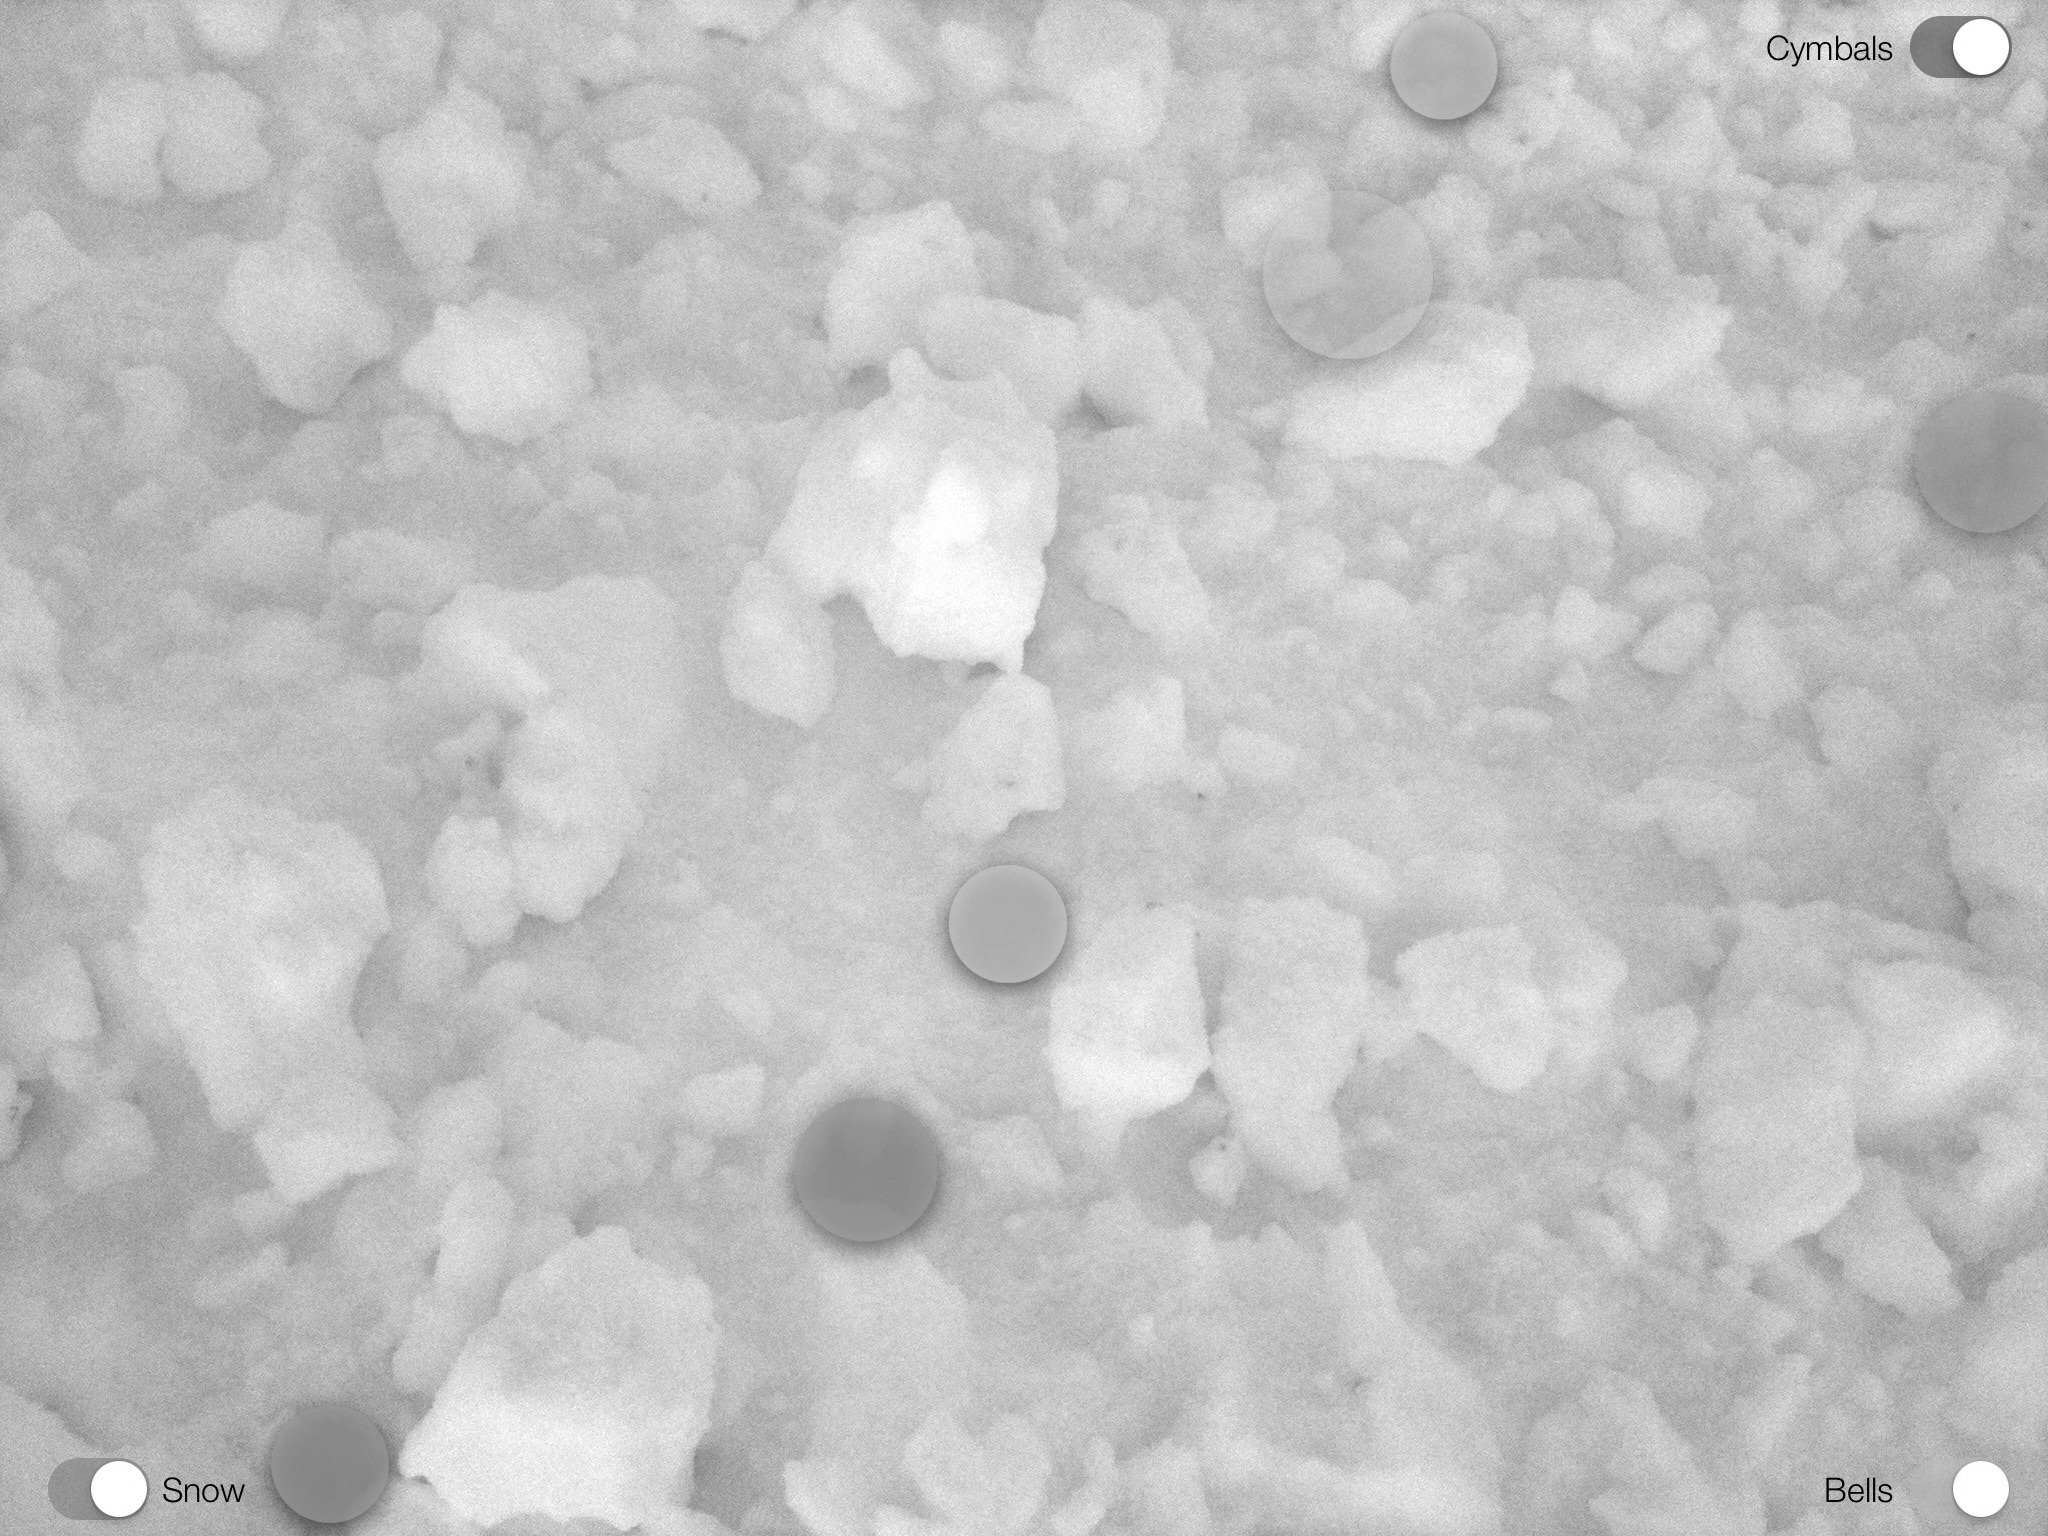
\includegraphics[width=0.45\textwidth]{figures/app-4-SnowMusic-bw}
  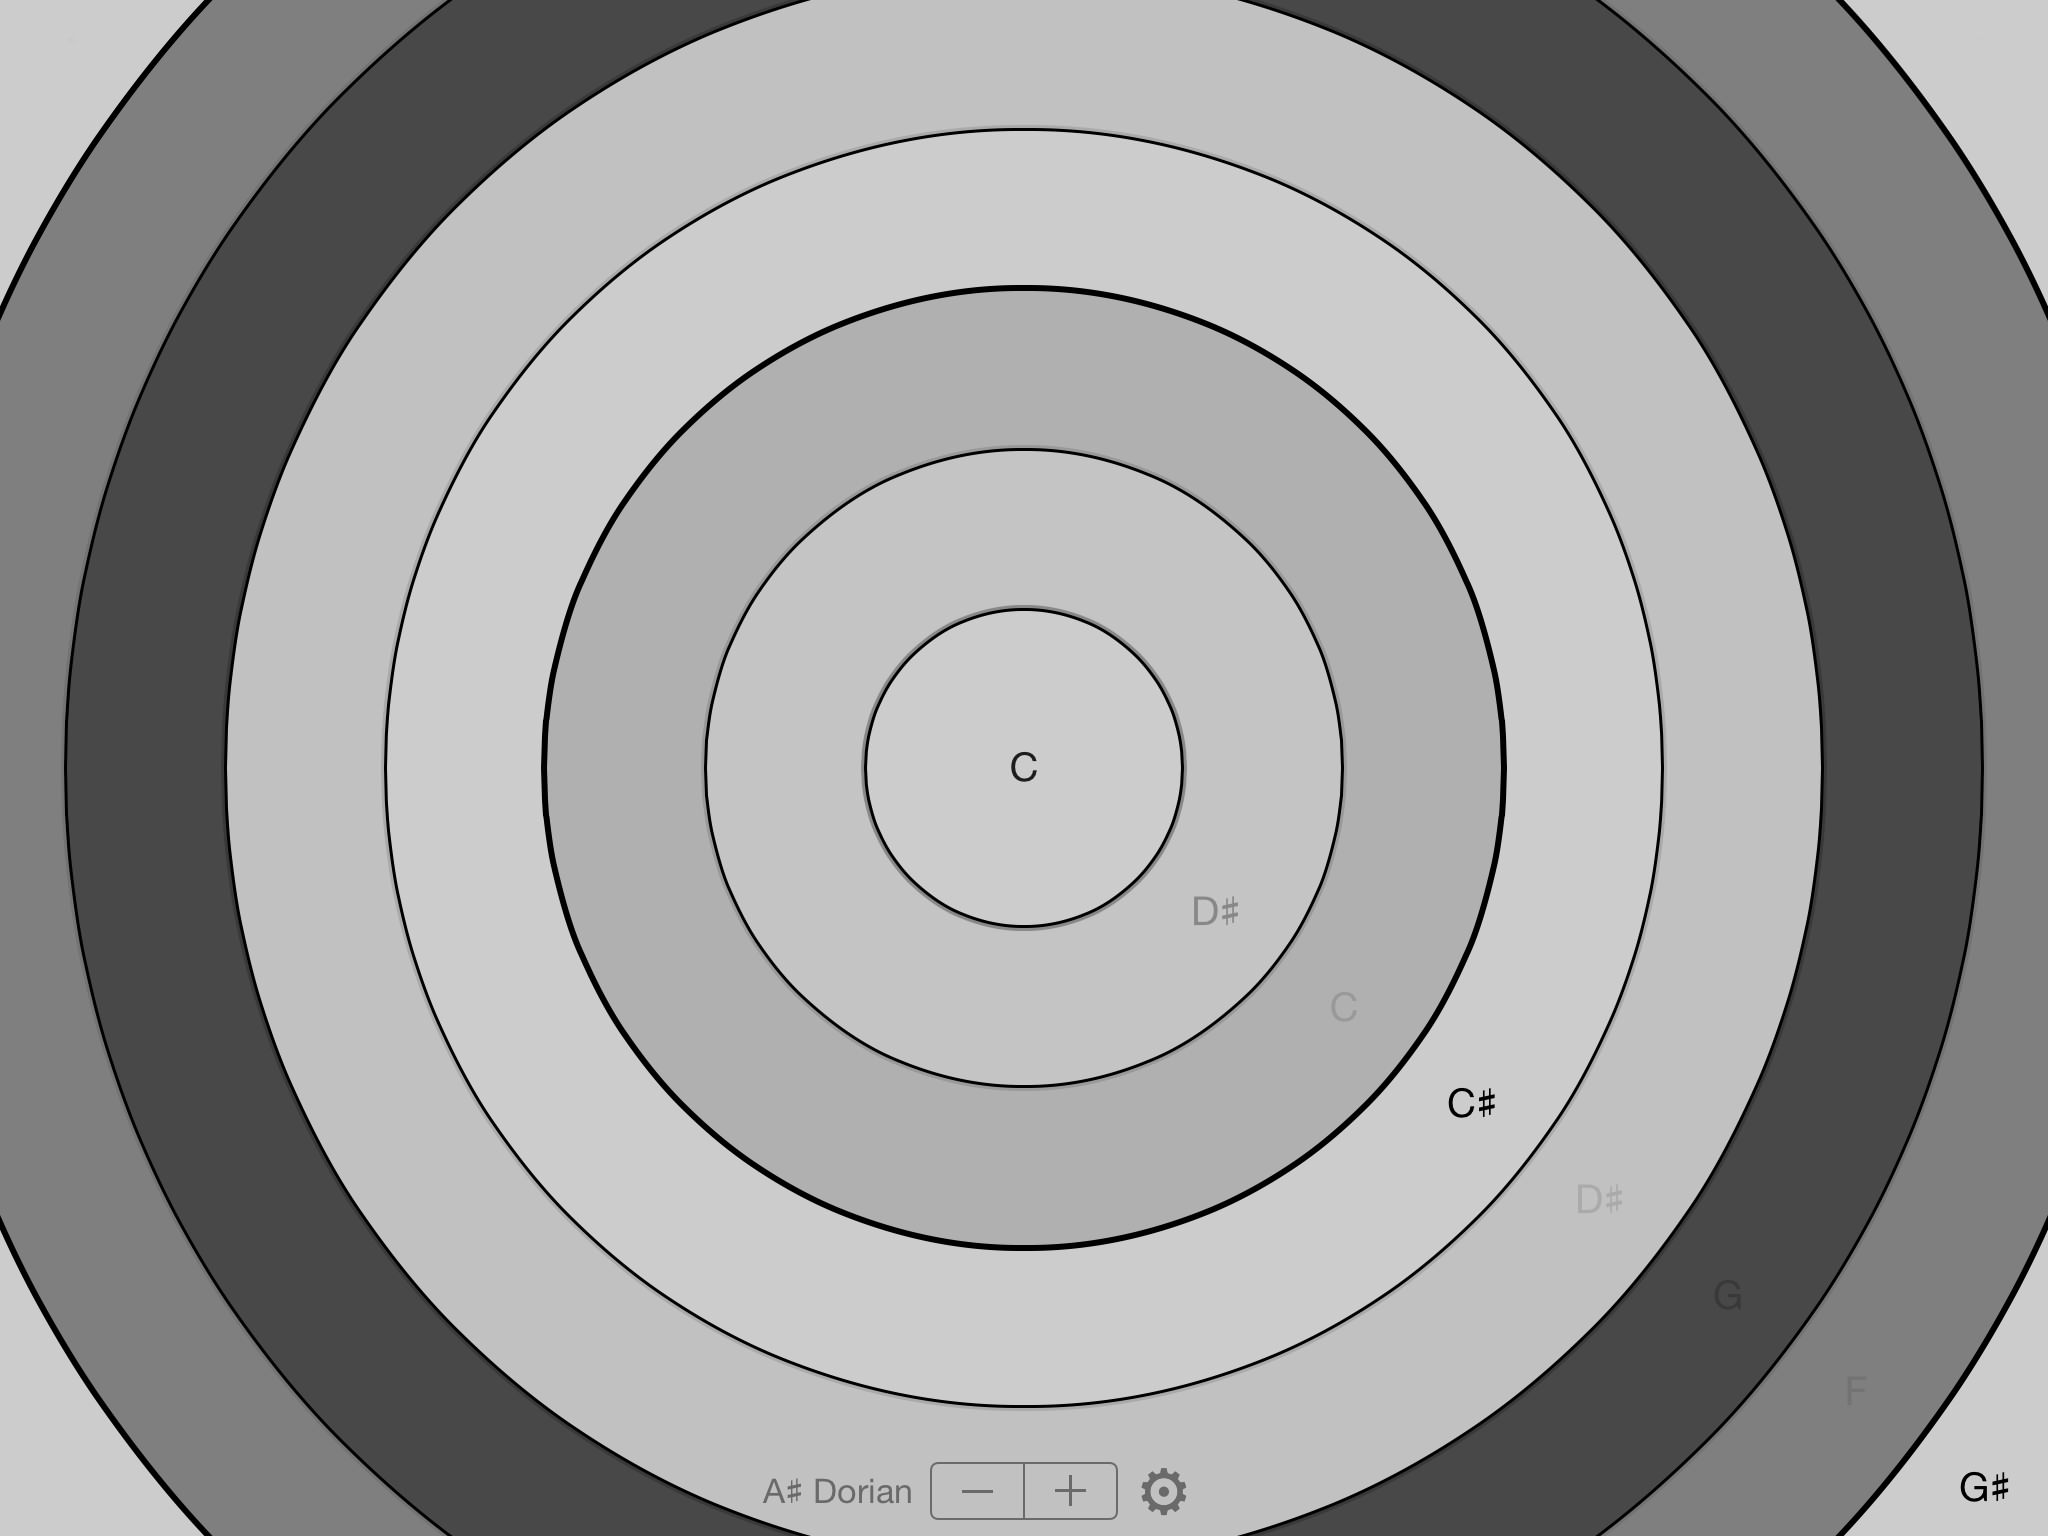
\includegraphics[width=0.45\textwidth]{figures/app-5-PhaseRings-bw}
\end{center}
\caption{Screenshots of four Metatone apps: \emph{MetaLonsdale},
  \emph{BirdsNest}, \emph{Snow Music}, and \emph{Phase Rings}.
  \emph{MetaLonsdale} and \emph{BirdsNest} allow free-form touch
  improvisation over the whole screen with a looping function that
  repeats tapped notes. \emph{Snow Music} allows performers to create
  snow sounds supported by alorithmically generated sound-scapes.
  \emph{PhaseRings} is an annular interface for performing with
  pitched percussion sounds selected from configurable scales.}
\label{fig:metatone-apps}
\end{figure}

The touch-screen device chosen for our performances was the Apple
iPad. A variety of apps, including four shown in Figure
\ref{fig:metatone-apps}, have been developed so far for performances
with Ensemble Metatone and other groups. All of the Metatone apps
share the same fundamental mode of interaction: a tap triggers a
single sound with a percussive envelope (i.e. a sharp attack and long
decay), while swiping plays a continuous sound with volume related to
the velocity of the moving touch. Apart from this commonality, the
Metatone apps feature different palettes of available sounds and modes
of synthesis, different arrangements of sounds on screen, a variety of
special features, and different kinds of networked interactions
between the iPads themselves as well as with a server application.

The earliest Metatone apps, \emph{MetaTravels} and \emph{MetaLonsdale}
were both designed to allow percussionists to control combinations of
field-recordings and pitched percussion
instruments~\cite{Martin:2014xp}. \emph{MetaTravels} used
field-recordings from around the world and all chromatic pitches were
available in the interface simultaneously. \emph{MetaLonsdale} limited
performers to field-recordings from a Canberra caf\'e and pitches from
a rotating sequences of scales. A related app, \emph{BirdsNest},
allowed performers to create a soundscape reminiscent of northern
Swedish forests, with samples of bird calls and field recordings from
the location as well as xylophone and woodblock samples. These three
apps used UI switches to control a looping feature that would repeat
tapped notes and UI buttons to shuffle the sounds available to the
player from a palette of sonic material. \emph{Snow Music} allows
percussionists to manipulate samples of snow sounds (similarly to
Burtner's amplified snow) and was originally developed with the
percussion group \emph{Ensemble Evolution}~\cite{Martin:2012fk}. The
app allows performers to switch on algorithmically produced backing
soundtracks to accompany themselves. \emph{PhaseRings} is the latest
Metatone app and consists of an annular interface for performing with
pitched percussion sounds. Each ring in the interface corresponds to a
different pitch, performers configure the app with a sequence of
musical scales and the app displays a subset pitch-rings taken from
those scales with changes in the ring setup triggered by network
interactions or UI elements\footnote{The Metatone apps are available
  on the iTunes apps store and links can be found on
  \url{http://metatone.net}. This website also includes videos and
  audio recordings of performances with these apps.}.

In performances with our iPad apps, all touch interactions during the
performance are transmitted over a Wi-Fi network. Our server software
has evolved from a simple script in early rehearsals to a Python
server application, Metatone
Classifier\footnote{\url{http://metatone.net/metatoneclassifier/}},
that can run on a local network or on a remote virtual server.
Communications between the apps and server are accomplished using the
OSC~\cite{osc-nime2009} (Open Sound Control) message format. Data is
transmitted either through Unix sockets using the UDP protocol (as is
typical for OSC messages) or through WebSockets~\cite{Fette:2011eu},
which is the preferred method due to increased reliability of
transmission and the ability to easily open a bi-directional
connection with a remote server. The Metatone apps automatically find
the server and other active Metatone apps on their local network using
Bonjour (zero-configuration networking). The interactions between the
Metatone apps themselves and the apps and Metatone Classifier have
been documented elsewhere~\cite{Martin:2015mz,Martin:2015jk}. While
the designs of these interactions are outside of the scope of the
present chapter, it suffices to say that our goal has been to
introduce features that synchronise changes in the app's functionality
throughout performances in response to individual and ensemble
interactions. These features are designed to emphasise and enhance the
sense of group-mind that has been observed in performances of ensemble
free-improvisation~\cite{Borgo:2006fv}. 

\subsection{The Metatone Log Protocol}
\label{subsec:metatone-log}

Over our earliest rehearsals with Ensemble Metatone and the
\emph{MetaTravels} app, we developed a protocol for capturing
touch-screen information from each performer's iPad that mirrors Apple
iOS's touch-event handling framework. The information is sent to a
central server using the OSC data format. As we developed more
features for our apps and our server software, Metatone Classifier,
this protocol was extended to document the performers' gestural and
ensemble states and app-to-app interactions sent between iPads. A
complete listing of our OSC messaging scheme is given in Table
\ref{oscschema}. When our server receives one of these OSC messages,
it assigns a timestamp and records it to a text file for later
analysis. Each line of the text file is written in the CSV (comma
separated values) format. Although the different aspects of the
performance are recorded using different numbers of parameters, these
can be trivially separated or reorganised by filtering through the
unique OSC address of each type of message.

\begin{table}
  \begin{center}
  \begin{tabular}{|l|l|}
  \hline
  App to Server Messages: &\\
  \hline
  OSC Address           & Parameters \\ 
  \hline
  \texttt{/metatone/online}      & device  \\     
  \texttt{/metatone/touch}       & device, X, Y, velocity \\
  \texttt{/metatone/touch/ended} & device \\  
  \texttt{/metatone/switch}      & device, name, position\\
  \texttt{/metatone/app}         & device, name, state\\
  \hline
  % \end{tabular}\\
  Server to App Messages:&\\
  % \begin{tabular}{|l|l|}
  \hline
  OSC Address           & Parameters \\ \hline
  \texttt{/metatone/classifier/gesture} & device, gesture type\\
  \texttt{/metatone/classifier/ensemble/event/new\_idea} & device, measure value\\
  \texttt{/metatone/classifier/ensemble/state} & type, value 1, value 2 \\
  \hline
  \end{tabular}
\end{center}
\caption{Scheme for OSC messages from the Metatone iPad apps. The
  touch and touch ended messages record touch screen interactions
  directly from the iOS operating system (see Figure
  /ref{touch-event-code-listing}. 
  The ``device'' parameters are unique identifiers for each iPad in
  the ensemble.
}
\label{oscschema} 
\end{table}

Our iPad apps send messages to the server in response to three of the
four touch-events in iOS, \texttt{touchesBegan},
\texttt{touchesMoved}, and \texttt{touchesEnded}. Both the beginning
and movements of touches are recorded using a \texttt{/touch} message
recording the iPad's app-level unique device ID. The velocity of
\texttt{touchesMoved} messages is recorded while \texttt{touchesBegan}
messages are distinguished by having a velocity of zero. A
\texttt{/touch/ended} message is used to record \texttt{touchesEnded}
events. \texttt{touchesCancelled} messages are ignored.
 
Each of our iPad apps contains a small number of button and switch UI
elements that are used in the performances to activate looping
functions, algorithmically generated backing sounds, and to change the
timbre and pitch of sounds available through the touch interface. The
performers' interactions with these elements are recorded using
\texttt{/switch} messages which record the iPad device ID, the name of
the UI element and its new state. During performances, our iPad apps
send messages to the other apps performing while connected on the same
local network. These messages are also copied to the server software
using the \texttt{/app} OSC address.

As will be described in later sections, Metatone Classifier has the
capacity to identify the performers' touch gestures in real-time
during performances. The server tracks these gestures to identify the
whole state of the whole ensemble and, in particular, identify moments
of peak gestural change where the group may have moved onto a new
musical section. While this information is recorded for later
analysis, it is also returned to the performers' apps, which use it to
update their interfaces and present new performance possibilities to
the performers~\cite{Martin:2015jk}. Our protocol for performance
logging includes three OSC messages from the server to the iPad apps.
Gesture classifications are returned to the iPads each second with OSC
\texttt{/gesture} messages; whenever a new musical section is
detected, the server sends an \texttt{/event/new\_idea} message to all
connected iPads. Various measures of the ensemble state are
returned to the iPads each second using the OSC address,
\texttt{/state}.

This scheme for logging touch-interactions (see Table \ref{oscschema})
was chosen to study the process of improvising with iPad instruments
and not necessarily for replaying performances. Other aspects of the
touch-screen state, such as unique identifiers for each touch point, are
not tracked, nor are the exact pitches available on screen for each
player. Multitracked audio recordings of performance are deemed to be
sufficient record of the particular sounds created during the
performance while the touch protocols store the details of performers'
interaction with the instruments that the audio recording cannot.
While our protocols were created for research purposes, the CSV
storage format allows us to easily transform these logs into
alternative representations of performances. The next section will
describe these new outputs, and how they not only aid in understanding
the improvised performances, but serve as representative artefacts
along with audio and video recordings.

\section{Transcoding Performance Protocols}
\label{sec:analysis}

Our system of iPad apps and server software records all touch events,
UI interactions, and app-to-app communications that occur during
improvised performances and records them in CSV format. These
recordings are mutable new-media objects and, as suggested by Manovic,
by transcoding these objects ``the logic of a computer can be expected
to significantly influence the traditional cultural logic of
media''~\cite{Manovich:2002ly}.

In this section we will describe ways in which our performance
protocols can be transcoded into new representations of the
improvisations, both in real-time during the performance and
afterwards. We will explain how gestural classifications of each
performer's touches leads to graphical ``scores'' and animated
visualisations provide new perspectives on the ensemble interaction.
These representations not only form important archival documents of
performance but feed into the ongoing artistic practice of
touch-screen improvisation.

% Our server software analyses these gestures during the
% performance to produce more information about the performers'
% interactions with the touch-screen devices and the state of the whole
% ensemble. After performances, the touch protocols can be transformed
% into gestural ``scores'' of the improvised pieces and into animations
% of the performers' touch interactions. These representations of the
% performance form a detailed archive of our improvised musical practice
% and aid our efforts to analyse and understand touch-screen
% performance.

\subsection{Gesture Classification and Gestural Scores}
\label{subsec:gesture-classification}

Each second during performances, our server software analyses the
previous five seconds of touch-data from each connected iPad and
identifies the performers' current touch gesture. Our system
calculates feature vectors of descriptive statistics for each player
from these five-second windows of recorded touch interactions. The
feature vectors are classified using a Random Forest
Classifier~\cite{Breiman:2001kx} from the Python \texttt{scikit-learn}
library that is trained with examples of nine touch gestures recorded
by our app designer using a formal data collection
procedure~\cite{Martin:2015jk}. 

\begin{table}
\begin{center}
    \begin{tabular}{|l|l|l|l|}
    \hline
    \# & Code & Description & Group \\ \hline
    0 & N   & Nothing & 0 \\
    1 & FT  & Fast Tapping & 1\\
    2 & ST  & Slow Tapping & 1\\
    3 & FS  & Fast Swiping & 2\\
    4 & FSA & Accelerating Fast Swiping & 2\\
    5 & VSS & Very Slow Swirling & 3\\
    6 & BS  & Big Swirling & 3\\
    7 & SS  & Small Swirling & 3\\
    8 & C   & Combination of Swirls and Taps & 4\\ \hline
    \end{tabular}
\end{center}
\caption{The nine gesture classes that our server software, Metatone
  Classifier, can identify in touch screen performances. This
  vocabulary resembles the gestural language of percussion
  performance, rather than typical command gestures used in HCI.}
\label{tab:gesture-classes}
\end{table}


The nine gesture classes are based on those discovered through
qualitative analysis of Ensemble Metatone's earliest series of
rehearsals~\cite{Martin:2014jk}. The vocabulary focusses on three
fundamental touch gesture groups: tapping, swiping, and swirling, and
it includes several variations of each group. Unlike other systems for
gesture recognition~\cite{Wobbrock:2007kq} which are designed to
interpret sequences of movements with a beginning and ending as a
command in a computing interface\footnote{This includes Apple's built
  in \texttt{UIGestureRecognizer}~\cite{AppleDeveloper:2015rm}
  class.}, our classification system aims to segment a continuous
stream of free-form gestures. For this reason, our vocabulary seeks to
identify ``tapping'', which could continue indefinitely, rather than
``tap'' which is completed after one touch interaction. In this way,
our touch-screen gestural vocabulary resembles some of the snow
gestures of \emph{Syntax of Snow}~\cite{Burtner:2011fk} which also are
open ended with respect to the number or length of interactions.
Applying this gestural classification scheme to touch-screen
performances results in a new representation of the performance, that
is, a time series of gesture classes at one-second intervals for each
performer in the ensemble. Although this time series does not contain
the details of each performer's interactions, it can still serve as a
kind of musical score for performances, albeit a non-traditional one.

When a graphical plot is created of such a time series, the score
starts to bear resemblence to the time-space graphical scores of
contemporary classical music. In the gesture-score plots of Figure
\ref{gesturescore}, each performer's gestures are represented by a
different coloured line. These gesture-scores reveal much about the
structure of improvisations that is difficult to appreciate from
temporal representations like audio and video recordings. In Figure
\ref{gesturescore}, it is clear when all performers are focussed on
the same broad gesture groups as their lines are on close levels of
the plot. When one performer breaks out for a solo idea, their line
moves up or down, or might move to the ``nothing'' level if they 
have stopped playing. Sometimes the performers split into
sub-ensembles, exploring separate groups of gestures. Perhaps most
interesting are the broadest structural elements where all members of
the ensemble change gestures together over a short period of time.
Such moments of increased change seem to segment the improvisations
into large sections. In a composed piece, these might be called
movements, but in an improvised setting, they appear to be related to
``new idea'' moments where the ensemble spontaneously transitions into
a different sound or musical behaviour. While such behaviour in
improvisation has been previously described by by
Pressing~\cite{Pressing:1988uo}, Stenstr\"om~\cite{Stenstrom:2009xy},
Bailey~\cite{Bailey:1993zl}, and others, it has not previously been
observed in an automatically-generated gestural transcription.

Since these gestural scores are so helpful in understanding, at a
glance, the overall flow of improvised touch-screen performances, they
serve as more useful archival documents of performances than, for
example, still photographs of the stage setup. Rather than simply
recording the location and setting of the performers, gesture scores
store a high-level view of the performers' gestures throughout a whole
performance. In fact, it would be possible to use gesture scores as
the reference material for new musical performances. An ensemble of
touch-screen musicians could simply read a gesture-score, as they
would a graphical score, and play through the sequence of gestures.
Alternatively, a computerised score display with a synchronised cursor
could be used to assist the performers or even be integrated into the
touch-screen interface as in the Decibel
ScorePlayer~\cite{Hope:2015lr}. While such performances would probably
not retain the sonic characteristics of the source improvisation, they
would include similar musical interactions between the members of the
ensemble and identical moments of structural change. By selectively
recording and regenerating multiple versions of a transcribed gesture
score, a touch-screen ensemble could curate a repertoire of works from
improvised source material. This process has precedent in contemporary
classical music, the composer Stuart S. Smith recalls allowing
``muscle memory to create the initial gesture while letting my
mind/ear polish the gesture, refining cliches out of the
picture''~\cite{Smith:1998ff}.

% what are the other possibilities for using gestural scores?

\begin{figure}
\centering
%\includegraphics[width=0.9\textheight,angle=90,origin=c]{figures/Performance-14-03-17-18_09.pdf}
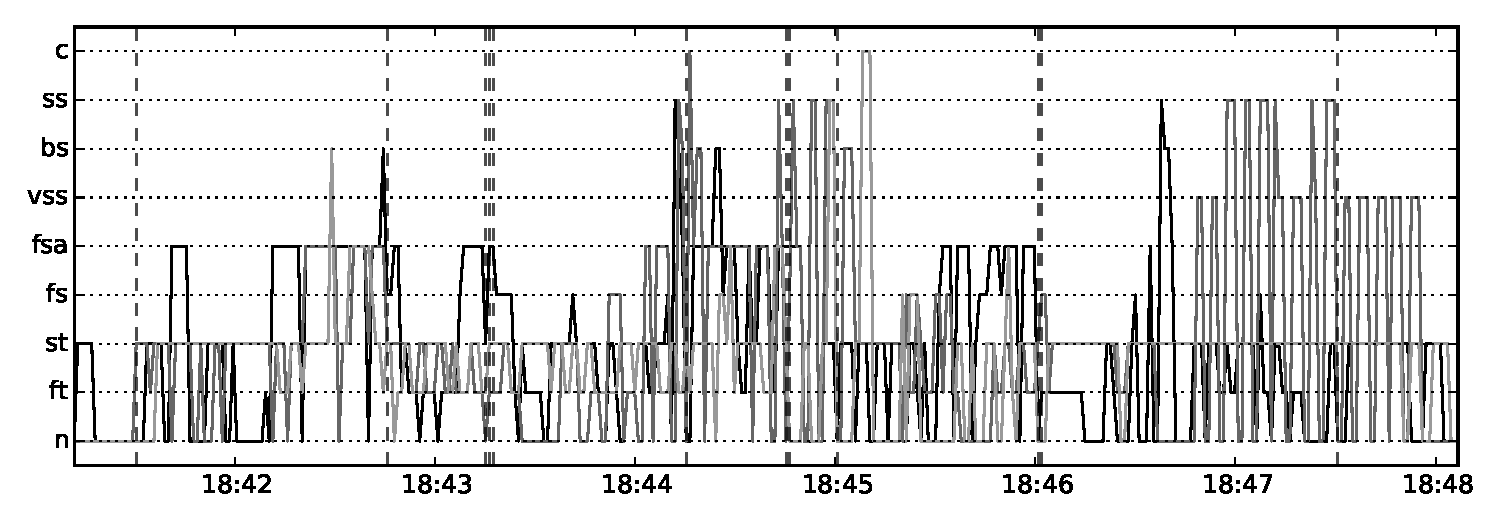
\includegraphics[width=0.9\textheight,angle=90,origin=c]{figures/Performance-14-08-14-18_40-bw.pdf}
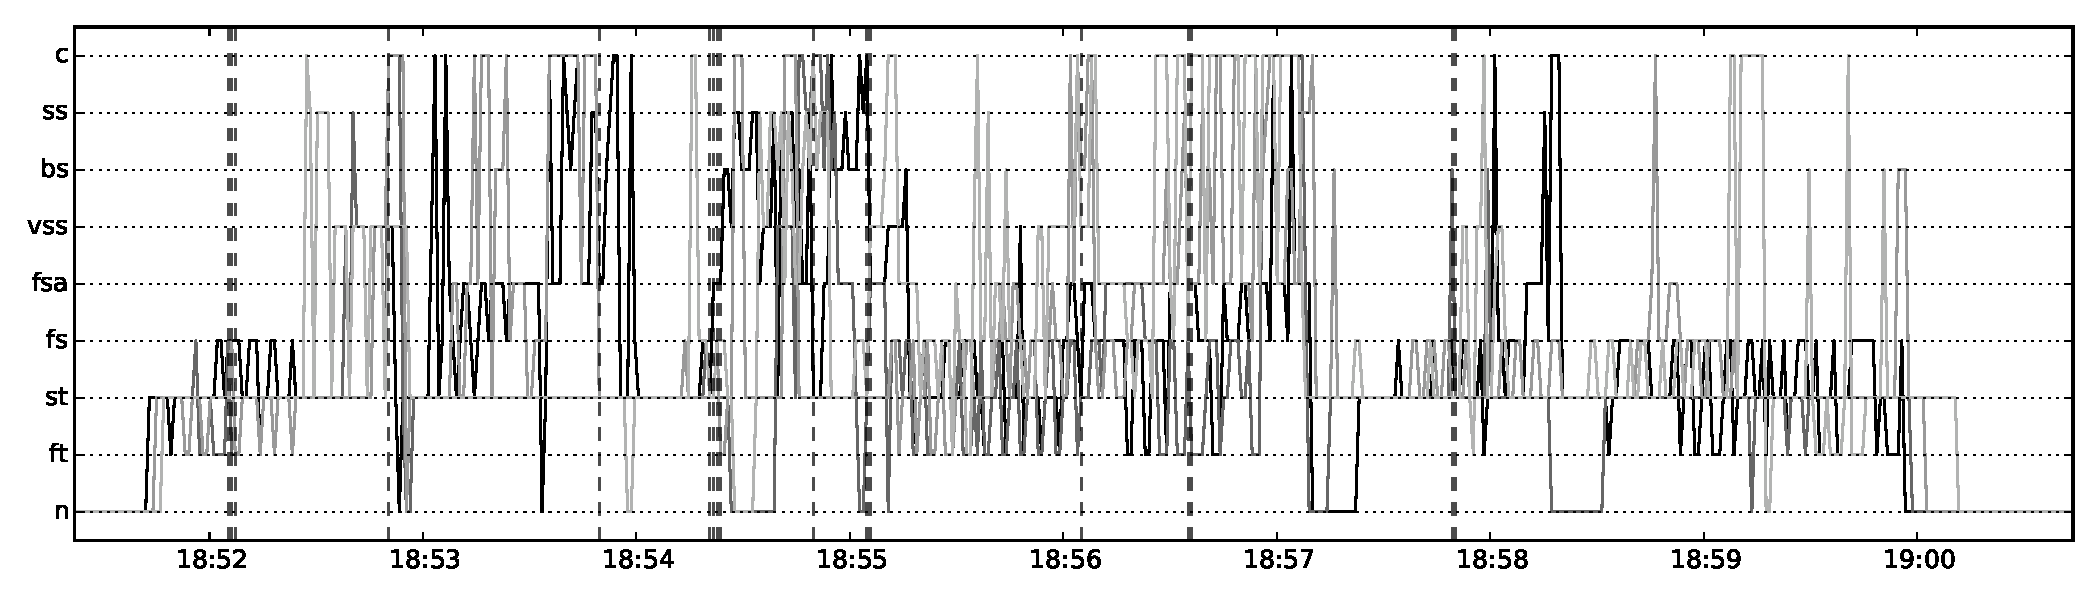
\includegraphics[width=0.9\textheight,angle=90,origin=c]{figures/gesture-score-15-05-07-18-52-bw.pdf}
%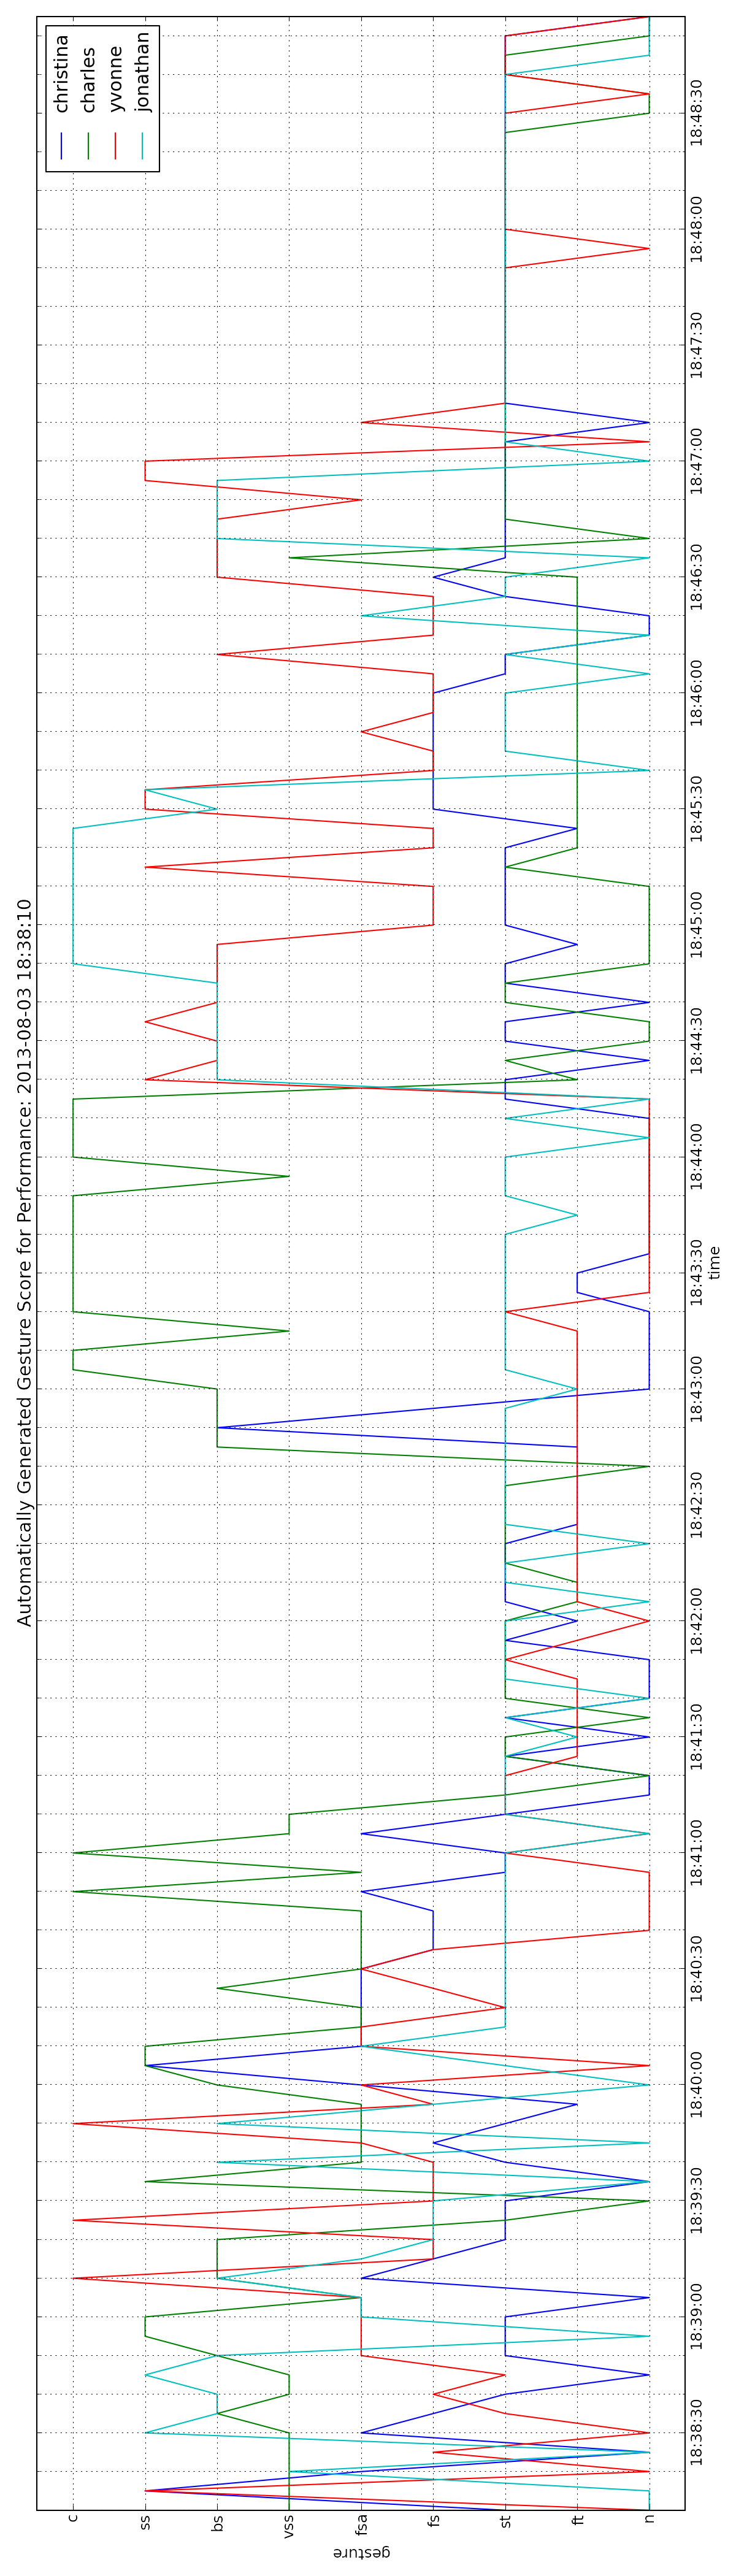
\includegraphics[height=0.9\textheight]{figures/score20130803vert}
%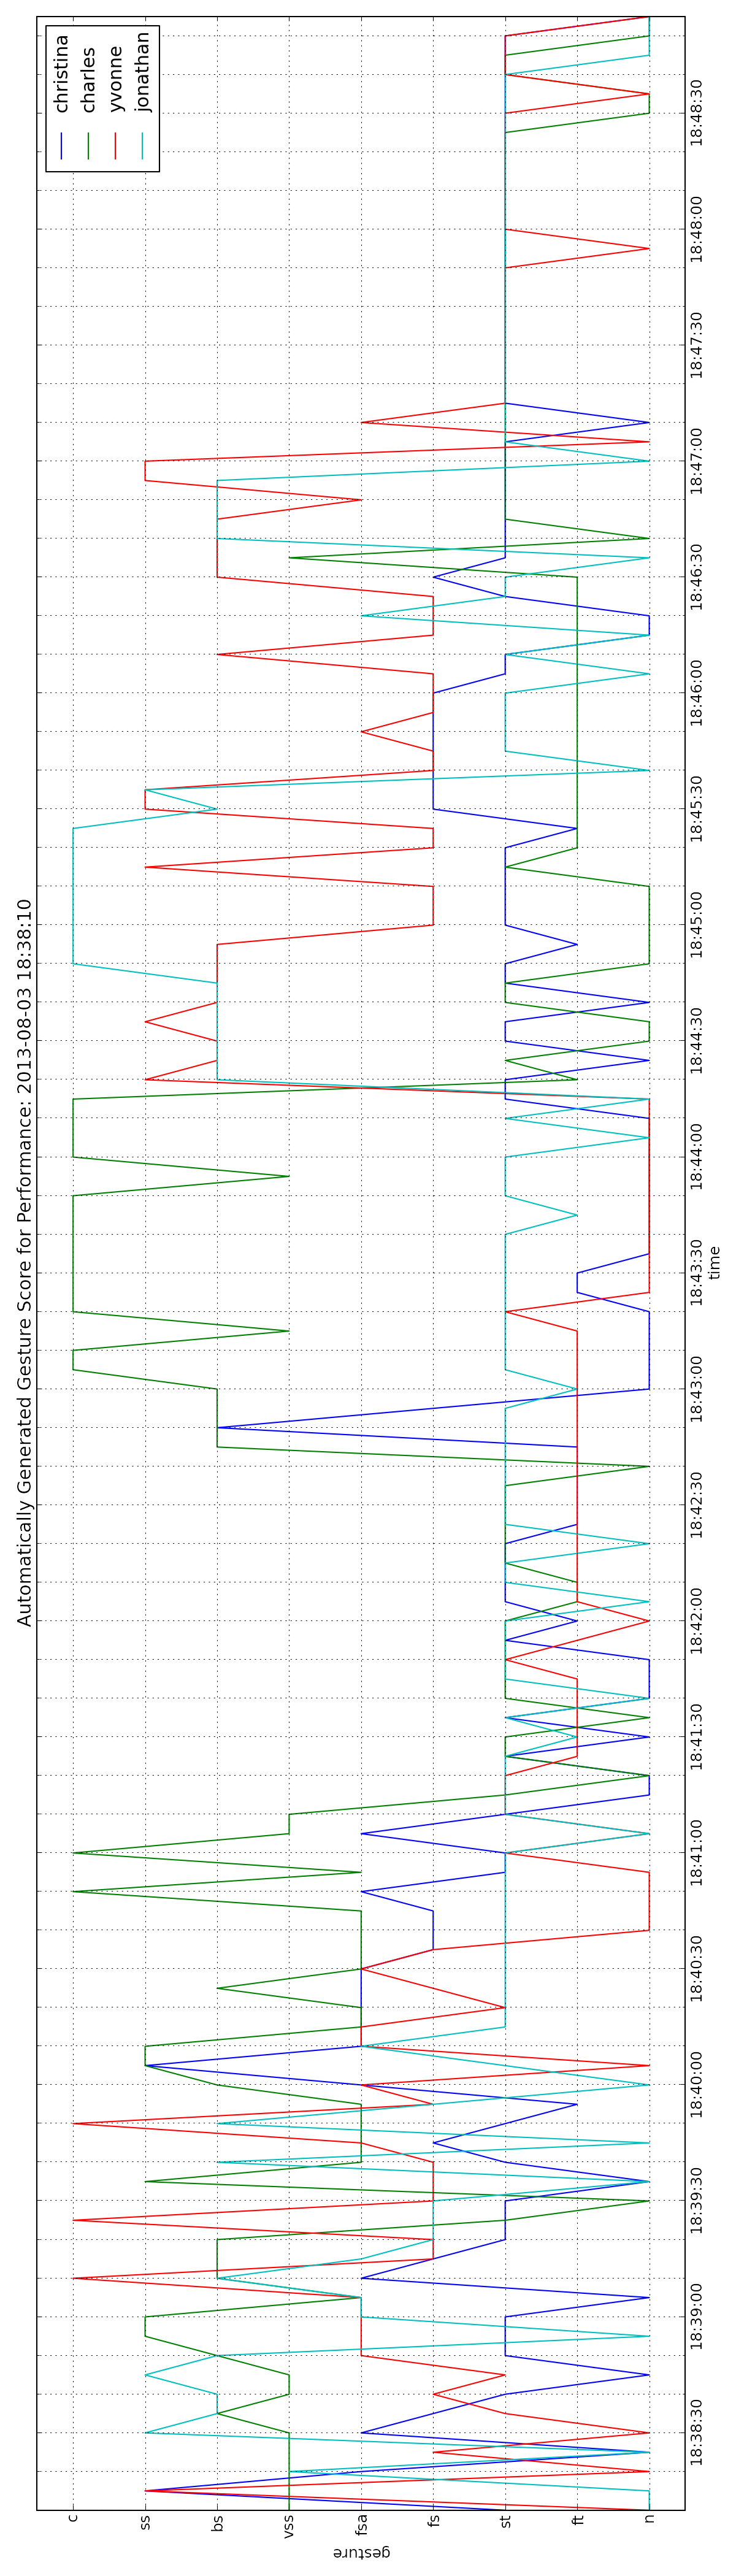
\includegraphics[height=0.9\textheight]{figures/score20130803vert}
\caption{Automatically generated gesture-score for two Ensemble
  Metatone performances in 2014. Each coloured line represents a
  single players' gestural classifications sampled once per second.
  The red dotted vertical lines represent moments when a new-idea
  message was triggered by the Metatone Classifier Server. The left
  score was a trio improvisation by Ensemble Evolution on 2014-08-14
  and the right score is of a quartet improvisation on 2015-05-07 by a
  group of research participants. See Table \ref{tab:gesture-classes}
  for definitions of the gestures given at each level of the y-axes.}
\label{gesturescore}
\end{figure}

% \subsection{Tracking Gestures as a Score}
% \label{subsec:gesture-scores}

\subsection{Identifying Special Events}
\label{subsec:special-events}

Some aspects of musical structure in touch-screen improvisations are
visually apparent in graphical gesture scores, but it is also possible
to automatically discriminate between different styles of touch-screen
performance and identify transitions between multiple sections. To
analyse such features, the performance of all performers in an
ensemble must be considered at once, and our time series of gestural
classifications are an ideal format for exploring these ensemble
interactions. The method used in our Metatone Classifier software is
that of transition matrix analysis~\cite{Swift:2014tya}, where
performers' changes between gestures are summarised in matrices
allowing simultaneous analysis of the whole ensemble over varying
windows of time, or over a whole performance. In Metatone Classifier,
transition matrices of gesture groups are calculated over 15-second
windows, each second during a performance, a value determined through
a process of trial and error. Once a transition matrix has been
produced, several measures can be applied to them with little
computational cost, an important factor in a real-time application.

Out of several experimental tests on transition matrices, our
\emph{flux} measure~\cite{Martin:2015jk} has proven to be extremely
promising. Flux is a measure of the rate of gestural change calculated
by dividing the number of transitions from one gesture to another by
the self-transitions where a gesture is followed by itself. The flux
of a transition matrix has a maximum of one, when no gesture follows
itself, and a minimum of zero, when each member of the ensemble stays
on the same gesture for the whole window of calculation. When applied
to a window of calculation that slides over a whole performance, peaks
in flux tend to match moments where the ensemble shifts to a new
section. In Metatone Classifier, we have implemented a strategy that
tracks sudden increases in flux to identify these new ideas.

When our software identifies one of these events during a performance,
an OSC message is sent to each of the connected iPad apps. We have
experimented with a number of responses in the app interfaces for
these messages~\cite{Martin:2015jk}. The apps might display a series
of new notes to reward the performers, or progress through a
composition of sound scapes to encourage further exploration.

As with all of our app-server interactions, new-idea messages are
logged to our performance protocols and have been useful in later
analysis of improvised performances. These messages are shown in
Figure \ref{gesturescore} as vertical red lines. Since calculations
over several seconds may identify the same increase in flux, new-idea
messages are often grouped together closely although our apps are
designed to ignore messages that arrive more frequently than once
every ten seconds. 

\subsection{Visualisations}
\label{subsec:visualisations}


\begin{figure}
  \centering
  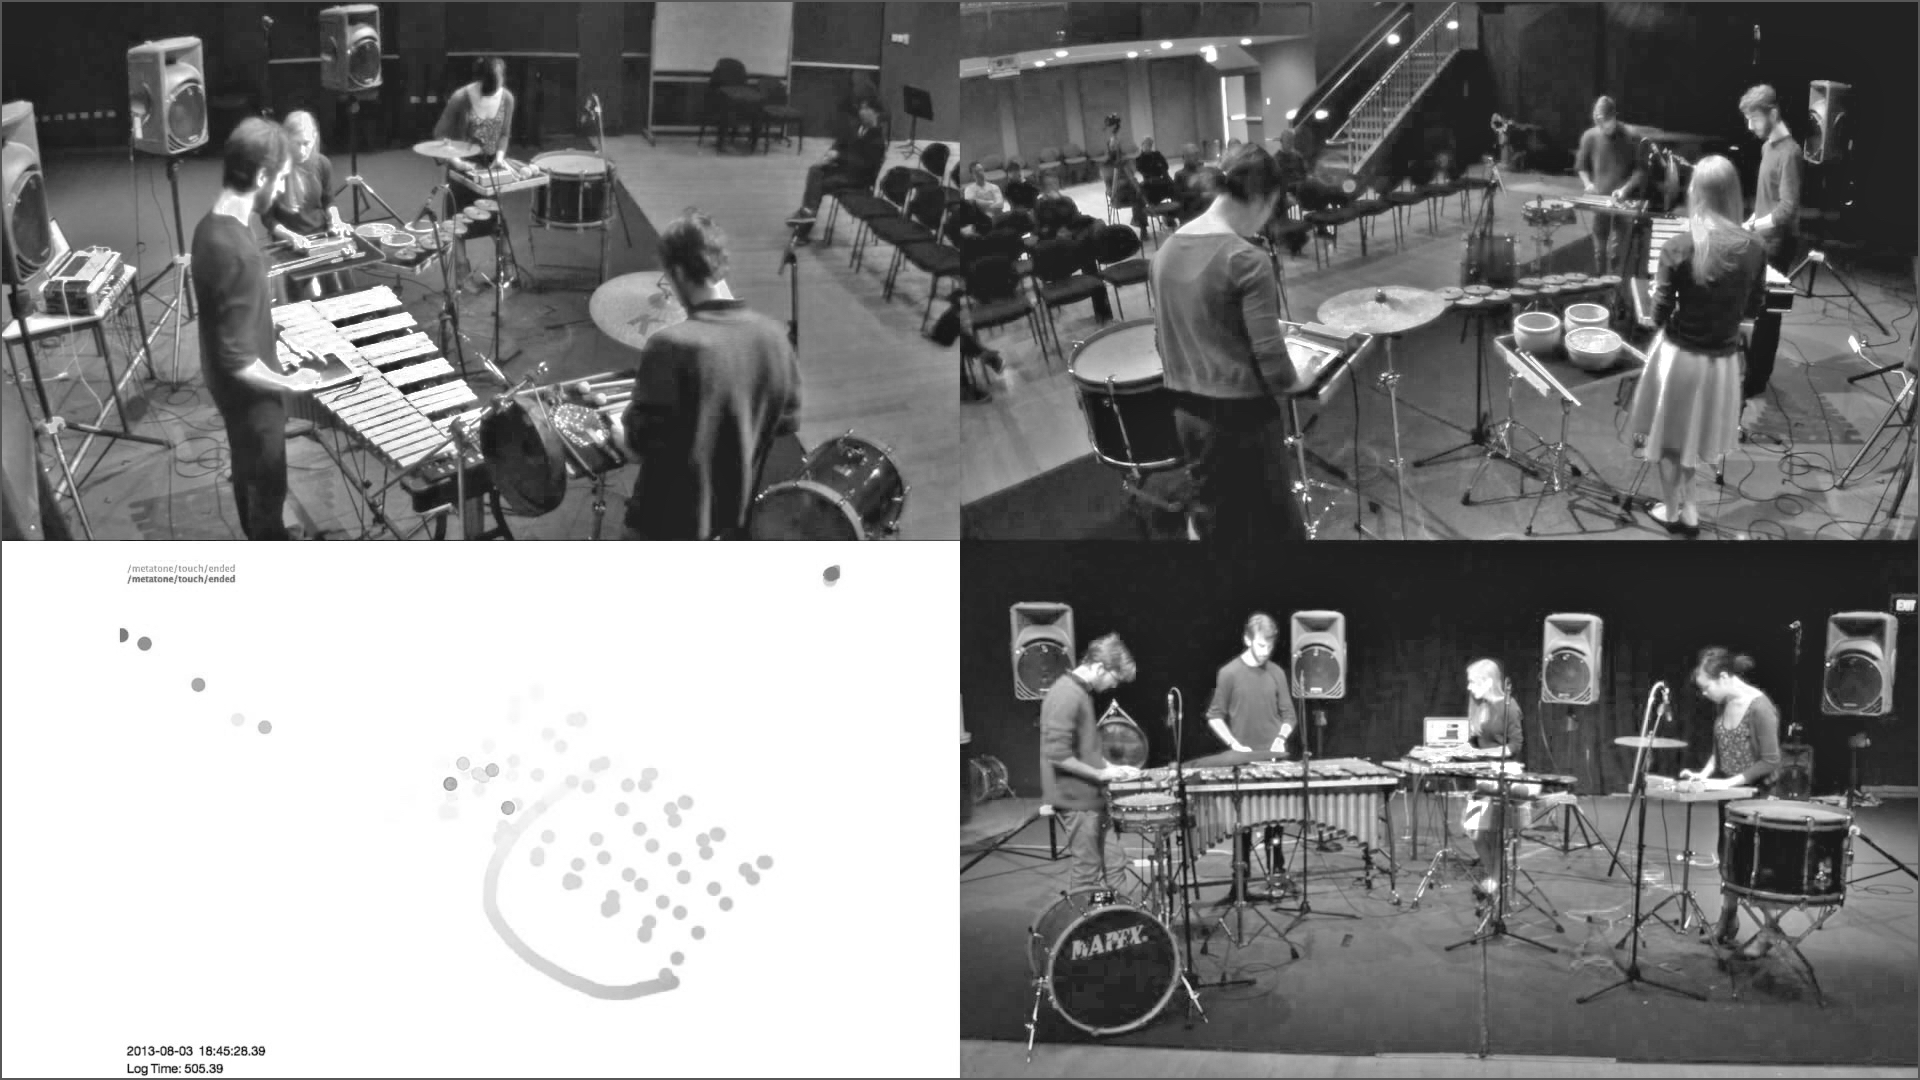
\includegraphics[width=0.9\textwidth]{figures/metatone-visualisation-metalonsdale-bw}
  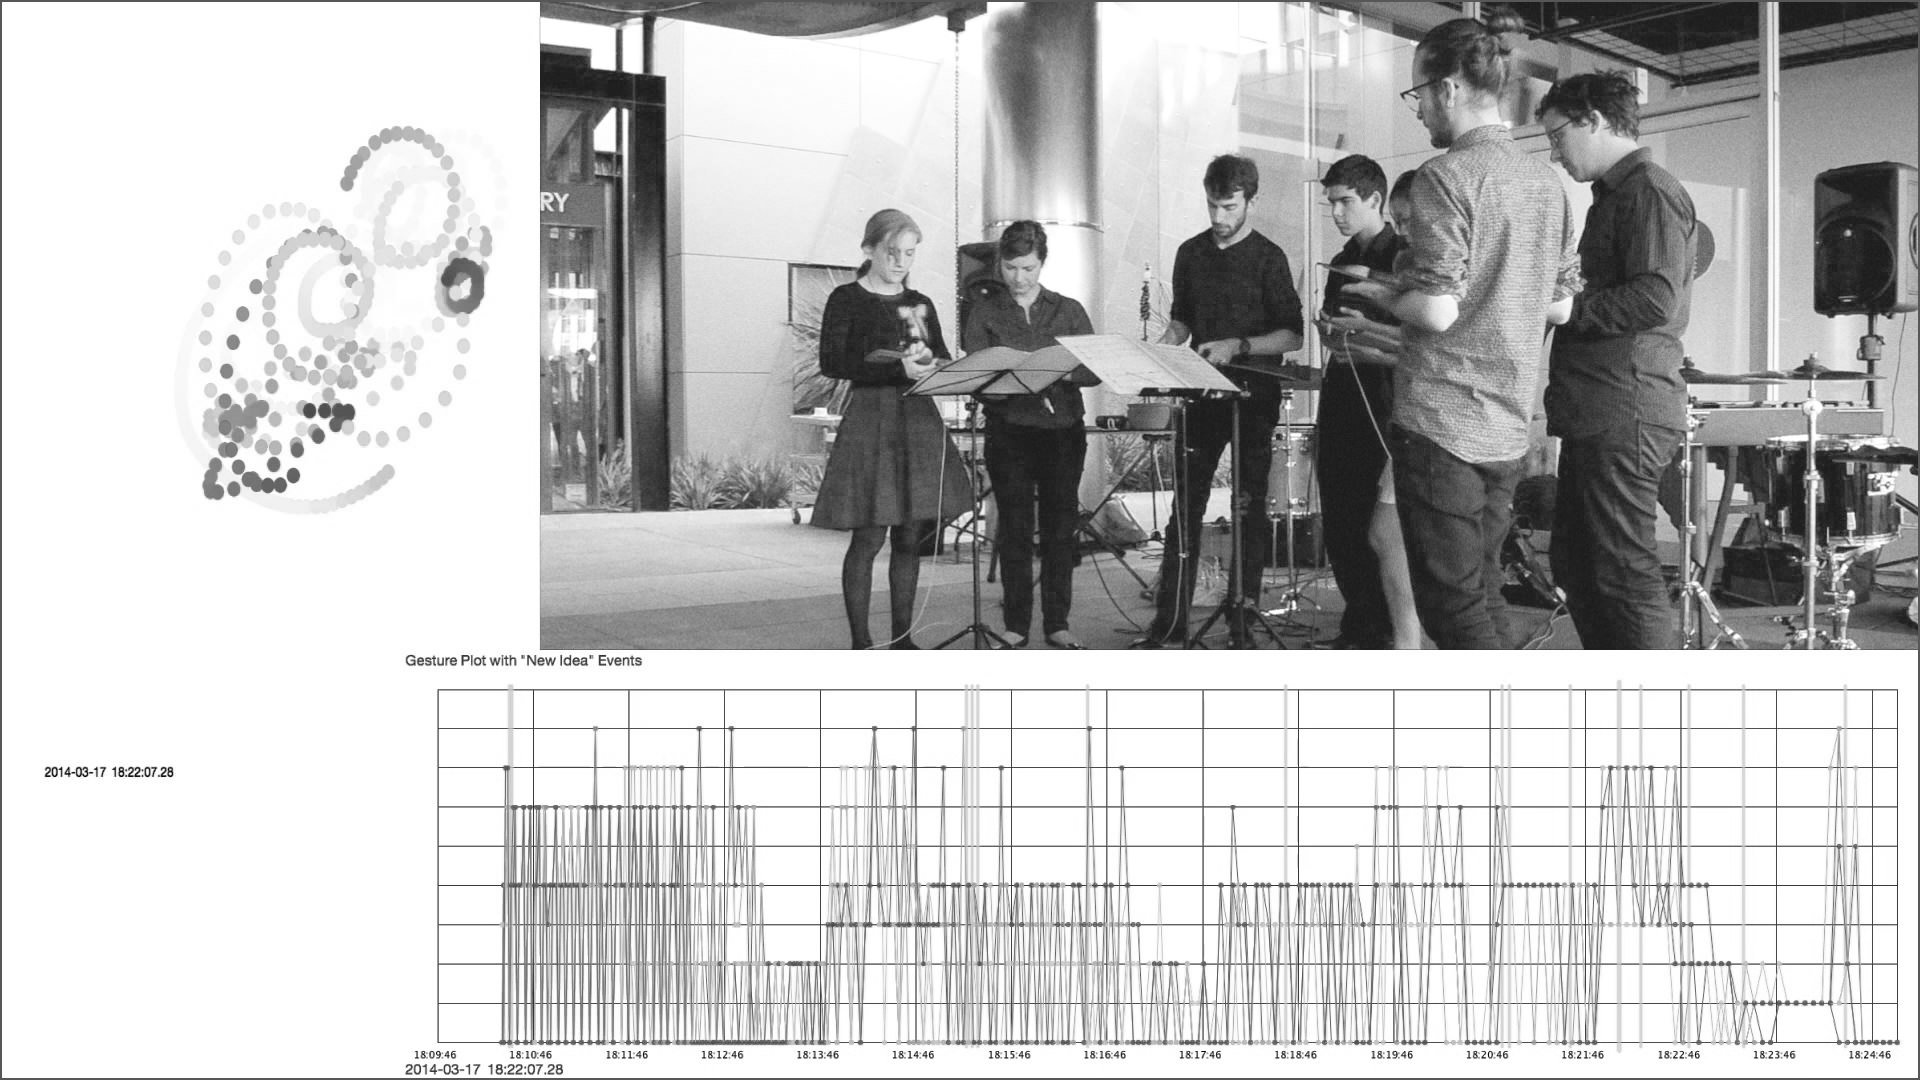
\includegraphics[width=0.9\textwidth]{figures/metatone-visualisation-youarehere-bw}
  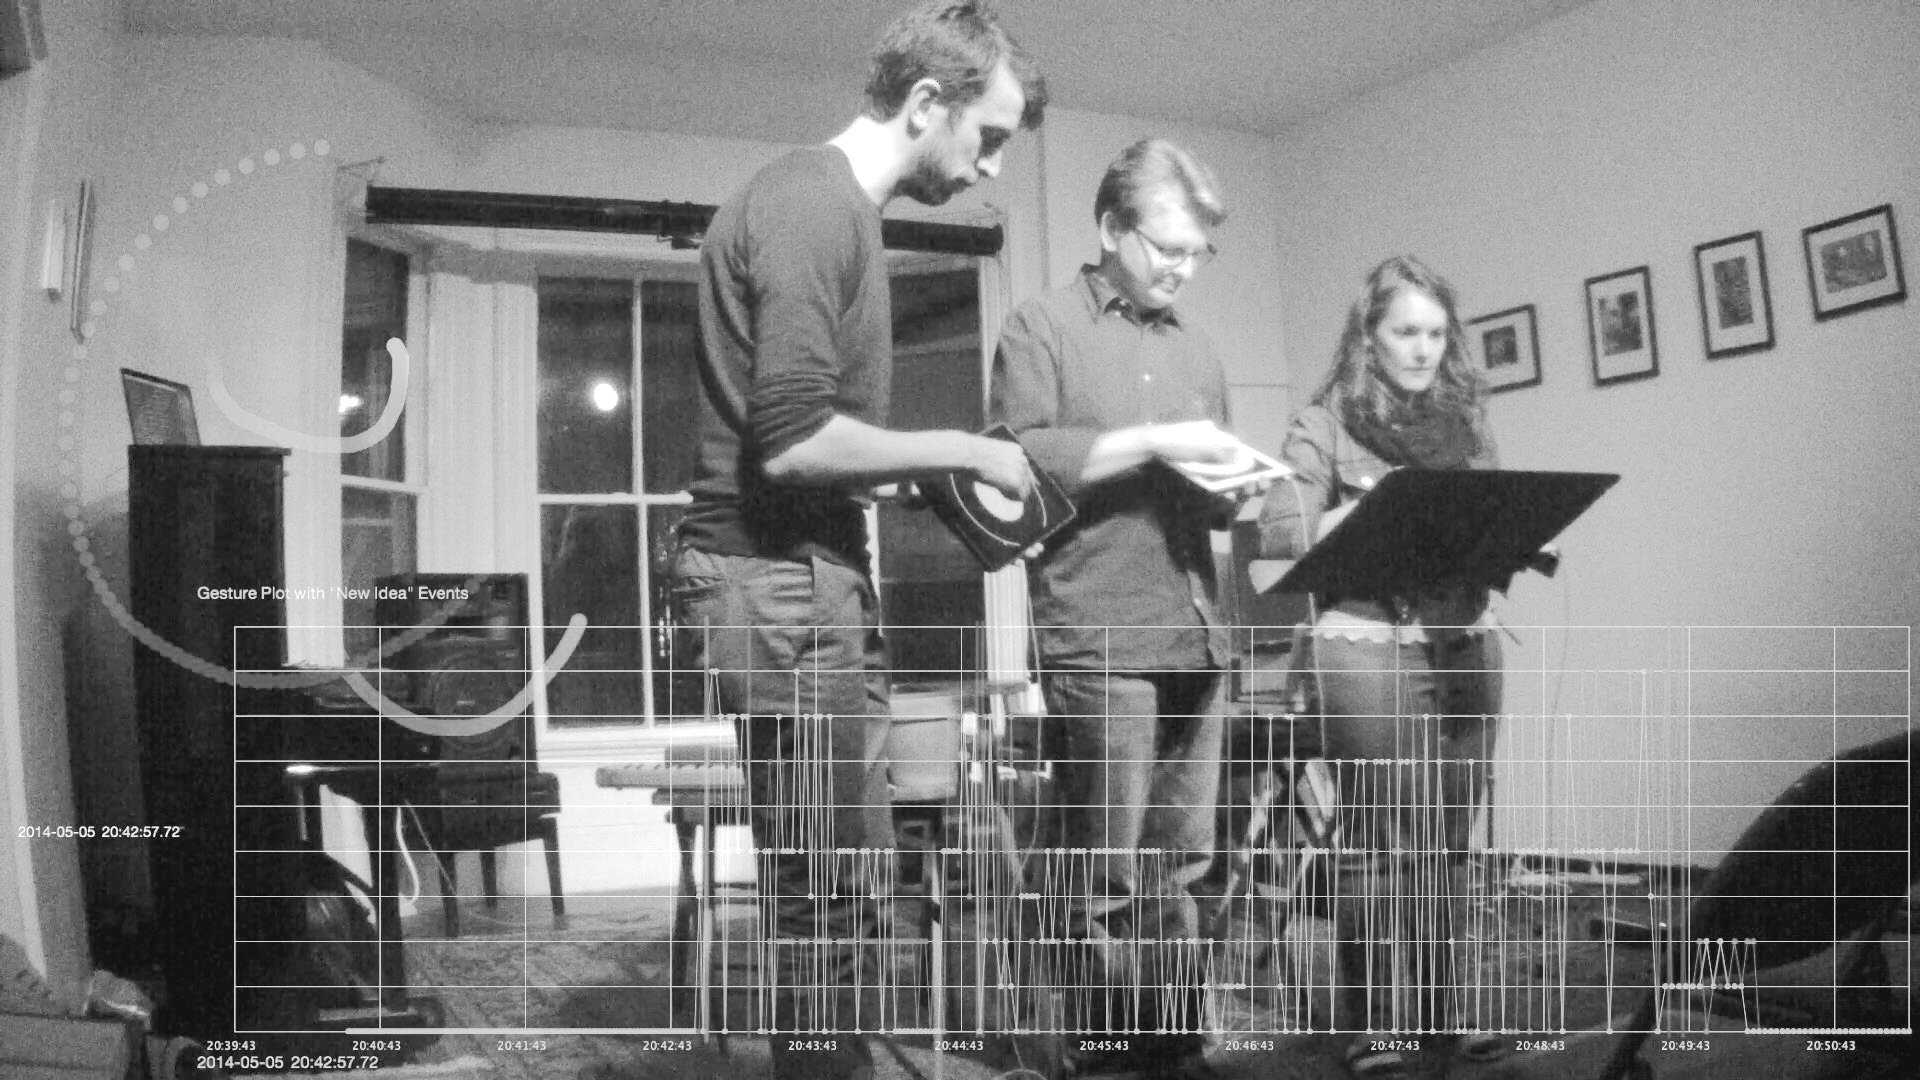
\includegraphics[width=0.9\textwidth]{figures/metatone-visualisation-touchandtone-bw}
  \caption{Stills from hybrid visualisations of three Ensemble Metatone
    performances showing video, touch animations, and gesture scores.
    From top to bottom, MetaLonsdale in Canberra, August 2013, Study
    in Bowls in Canberra, March 2014, and Touch and Tone in Boston,
    May 2014.}
  \label{fig:metatone-visualisations}
\end{figure}

To understand the structure of the improvised performances we have
developed method for translating touch and gesture protocols into
animated visual represenations of the performance that can accompany
the audio and video recordings in the documentation of each
performance. Two animations are typically produced for each
research-focussed performance one of the gesture classifications and
new-idea divisions and another for the performer's touches. The
Processing~\cite{Reas:2006kq} programming language has been used to
produce software that generates both animations.

The first visualisation is an animated version of the gesture-scores
discussed in Section \ref{subsec:gesture-classification}, with an
integrated playhead that indicates the current position in the
performance. The second animation visualises the logs of performers'
touches over each performance. Our program reads a captured log file
and renders an animation of all four players' touches overlaid in the
space of one iPad screen with the different players distinguished by
colour. Each touch point is represented by a circle that fades away
for about a second allowing different types of swirl, swipe, and tap
gestures to be distinguished at a glance. The software also draws a
date and time-stamp in each frame as well as text notification of app
and switch messages.

This touch animation presents an entirely new view of the
performance which was not visible to the performers or audience on the
day. As all the touch movements are layered in one performance area it
is immediately clear when performers mimic each other, form sections,
or experiment with a new musical idea. From the researcher's point of
view, the animation also gives a ``performer's perspective'' on touch
interaction, allowing us to connect patterns of touches with musical
gestures that the performers discuss after rehearsals.

While the two visualisations can be viewed separately, they are most
useful when synchronised with the audio and video recordings of
performances and displayed together. Figure
\ref{fig:metatone-visualisations} shows stills from hybrid
visualisations of three different performances. Each shows an
alternative arrangement of visualisations from our performance
protocols and multiple camera angles of video. Such videos have been
used within our research group to study the performances of Ensemble
Metatone and other groups that have performed with our iPad apps.
While the video component of these hybrid visualisations allows us to
recall the context of the concert and to observe the stage
interactions and communications of the performers, the visualised
touches and gestures have proven to be much more useful from a
research standpoint. With the gesture score we can see performance
interactions across time, and with the touch visualisation we can see
across the performers' touch spaces. In this way, the hybrid
visualisation becomes a kind of ``Seeing Space''~\cite{Victor:2014sf}
for improvised touch performances where multiple dimensions of the
performance can be examined simultaneously. This new and useful
representation of performances is only possible because of the
performance logging protocol that we have designed.

It is possible that these visualisations could also be used in a live
context where they are projected on large screen for the audience to
view or even superimposed on the performers' iPad touch screens. A
prototype touch visualisation has been developed from our software and
has been used as a backdrop projection in some performances, but the
implications and affordances of this addition to the performance have
not been fully explored.

\section{Conclusions}

In this chapter, we have presented our protocol for logging
free-improvised touch-screen musical performances which has been
implemented in our Metatone Classifier software and used to record
more than 80 performances by Ensemble Metatone and other groups. Our
protocol records all touch interactions during each performance as
well as network interactions between the performers' apps and the
server software. As each touch-interaction in our apps maps directly
to a sound and network interactions are key to our ensemble
improvisations, our protocol is a much more appropriate record of our
performance than other systems for tracking musical performances such
as MIDI. Our archive of performance protocols encode aspects of the
improvisations that are not accessible in traditional archives of
recordings and that align with theoretical models of free-improvised
music. They are also new-media objects satisfying Manovic's principles
for new media and can be transcoded into multiple alternative
representations of the performance. This leads to increased
understanding of touch-screen improvisation, the creation of
derivitive artworks, and informs the direction of future touch-screen
musical performances.

We have described our techniques for transforming logs into gestural
time series, graphical gesture-scores, and animated visualisations
that afford the viewer a new performer-centric perspective on the
touch improvisations. Animated visualisations have been crucial in
understanding the nature of touch-screen improvisation. These allow
the touches of all performers to be viewed simultaneously and clearly
show the vocabulary of gestures that the ensemble explores throughout
a performance. The time series of gestures have allowed us to perform
statistical investigations on the performances and uncover methods for
automatically segmenting performances by moments of gestural change.
Gesture-scores created by plotting these time series give an overview
of a whole improvised performance reminiscent of graphical scores.
These images allow multiple improvised performances to be directly
compared at a glance and could even be used as the stimulus for future
performances.

Importantly, these techniques have not just been used archive our
touch-screen performance but to develop an ongoing artistic practice.
This has included new Metatone apps that react to gestural
classifications and new-idea messages sent by the Metatone Classifier
server in real-time during performances, live visualisations of
touch-screen movements, and even compositions based on our vocabulary
of touch-screen gestures. While our touch-screen protocols allow
us to preserve past free-improvisations, they also suggest the form of
exploratory iPad performances of the future.

%\bibliographystyle{spphys}
\bibliographystyle{plain}
%\bibliographystyle{spbasic}
%\bibliographystyle{spmpsci}
\bibliography{2013ComputerMusic}
\end{document}

% %
% \section*{Appendix}
% \addcontentsline{toc}{section}{Appendix}
% %
% %
% When placed at the end of a chapter or contribution (as opposed to
% at the end of the book), the numbering of tables, figures, and
% equations in the appendix section continues on from that in the main
% text. Hence please \textit{do not} use the \verb|appendix| command
% when writing an appendix at the end of your chapter or contribution.
% If there is only one the appendix is designated ``Appendix'', or
% ``Appendix 1'', or ``Appendix 2'', etc. if there is more than one.
